\documentclass[11pt,a4paper,spanish]{book}
\usepackage{estilo_unir-1}
\usepackage[T1]{fontenc}
\usepackage{lmodern}
\usepackage{apacite}
\usepackage{array}
\usepackage{longtable}
\usepackage{booktabs}
\usepackage{multirow}
\usepackage{graphicx} % por si el estilo no lo carga; necesario para \resizebox e \includegraphics
\usepackage{tikz}
\usetikzlibrary{arrows.meta,positioning,shapes.geometric,fit,calc}
\usepackage{listings}
\usepackage{xcolor}

% Carpeta donde están las capturas de pantalla de la aplicación.
\graphicspath{{capts/}{./}}

% Estilo para los fragmentos de código fuente (Python).
\definecolor{codegris}{rgb}{0.95,0.95,0.95}
\definecolor{codecoment}{rgb}{0.40,0.45,0.50}
\definecolor{codeclave}{rgb}{0.10,0.25,0.55}
\definecolor{codestr}{rgb}{0.55,0.30,0.10}
\lstdefinestyle{python}{
  language=Python,
  basicstyle=\footnotesize\ttfamily,
  keywordstyle=\color{codeclave}\bfseries,
  commentstyle=\color{codecoment}\itshape,
  stringstyle=\color{codestr},
  numbers=left,
  numberstyle=\tiny\color{codecoment},
  stepnumber=1,
  numbersep=8pt,
  backgroundcolor=\color{codegris},
  showstringspaces=false,
  breaklines=true,
  frame=single,
  rulecolor=\color{codecoment},
  tabsize=4,
  captionpos=b,
  literate=%
    {á}{{\'a}}1 {é}{{\'e}}1 {í}{{\'i}}1 {ó}{{\'o}}1 {ú}{{\'u}}1
    {Á}{{\'A}}1 {É}{{\'E}}1 {Í}{{\'I}}1 {Ó}{{\'O}}1 {Ú}{{\'U}}1
    {ñ}{{\~n}}1 {Ñ}{{\~N}}1 {ü}{{\"u}}1 {¿}{{?`}}1 {¡}{{!`}}1
    {≤}{{$\leq$}}1 {Σ}{{$\Sigma$}}1
}
\lstset{style=python}

\numberwithin{equation}{chapter}
\numberwithin{figure}{chapter}
\numberwithin{table}{chapter}

% Comando auxiliar para la línea de fuente bajo los caption (no aparece en los índices).
\newcommand{\fuente}[1]{\par\vspace{2pt}{\footnotesize\textit{Fuente: #1}}}

%---------------------------
% Título del trabajo y autor
%---------------------------
\title{Sistema inteligente para la optimización de designaciones arbitrales en el voleibol}
\titulacion{Máster en Inteligencia Artificial}
\author{Adrián Estrada González}
\date{14 de abril de 2026}
\director{José Ángel de Bustos Pérez}
\nombreciudad{Siero, Principado de Asturias}

\begin{document}
\renewcommand{\listfigurename}{Índice de Ilustraciones}
\renewcommand{\listtablename}{Índice de Tablas}
\renewcommand{\contentsname}{Índice de Contenidos}
\renewcommand{\figurename}{Figura}
\renewcommand{\tablename}{Tabla}

\maketitle

\frontmatter
\tableofcontents
\listoffigures
\listoftables

%==================================================
\chapter{Resumen}

Cada fin de semana la Federación de Voleibol del Principado de Asturias (FVBPA) tiene que repartir a sus árbitros entre más de cien partidos, y hoy lo hace a mano. Es un trabajo largo, repetitivo y propenso a errores: hay que mirar a la vez quién está disponible cada día, qué nivel tiene cada árbitro, cómo se desplaza, evitar que pite partidos de su propio club y, encima, intentar que nadie se pegue viajes absurdos ni acabe con muchos más partidos que el resto.

Este Trabajo de Fin de Máster aborda ese problema, que en la literatura se conoce como \emph{Referee Assignment Problem} y se sabe que es NP-completo. La propuesta es un sistema que automatiza la designación arbitral combinando tres técnicas en una sola tubería: una heurística golosa que construye una primera solución válida, el solver exacto CP-SAT de Google OR-Tools, que la optimiza respetando todas las restricciones duras, y una búsqueda local que pule el resultado final. Sobre ese motor he montado una aplicación web completa, con su backend en FastAPI y una interfaz desde la que la federación gestiona árbitros, disponibilidad, calendario y categorías, lanza la asignación de un rango de fechas y revisa el resultado antes de publicarlo.

El sistema modela de forma explícita la disponibilidad por franjas, los niveles arbitrales, los solapes horarios teniendo en cuenta el tiempo de viaje, los conflictos de interés, el reparto equitativo y una idea de coche compartido que permite que un árbitro con vehículo recoja a un compañero que vive cerca. Probado con datos reales de la federación, sobre una jornada de 128 partidos alcanza una cobertura del 90\,\% de los roles en pocos segundos y reduce de forma notable los kilómetros frente a la asignación manual, demostrando que un enfoque híbrido de optimización e inteligencia artificial resuelve el problema de manera práctica.

\vspace{0.5cm}
\noindent{\bf Palabras Clave:} asignación de árbitros, optimización combinatoria, programación con restricciones, CP-SAT, voleibol, programación deportiva.

%==================================================
\chapter{Abstract}

Every weekend the Volleyball Federation of the Principality of Asturias (FVBPA) has to assign its referees to more than a hundred matches, and it still does so by hand. It is a long, repetitive and error-prone task: one has to consider at the same time who is available each day, the level of every referee, how each one travels, avoid having someone officiate matches involving their own club and, on top of that, try to keep travel reasonable and the workload balanced.

This Master's Thesis tackles that problem, known in the literature as the \emph{Referee Assignment Problem}, which is NP-complete. The proposal is a system that automates referee assignment by combining three techniques in a single pipeline: a greedy heuristic that builds a first feasible solution, Google OR-Tools' exact CP-SAT solver, which optimises it while respecting all hard constraints, and a local search that refines the final result. On top of that engine I have built a complete web application, with a FastAPI backend and an interface through which the federation manages referees, availability, the fixture calendar and categories, runs the assignment for a date range and reviews the result before publishing it.

The system explicitly models availability by time slots, refereeing levels, time overlaps accounting for travel time, conflicts of interest, fair workload distribution and a car-sharing idea that lets a referee with a vehicle pick up a colleague who lives nearby. Tested with real federation data, on a round of 128 matches it reaches 90\,\% role coverage in a few seconds and markedly reduces total kilometres compared with manual assignment, showing that a hybrid optimisation and artificial intelligence approach solves the problem in a practical way.

\vspace{0.5cm}
\noindent{\bf Keywords:} referee assignment, combinatorial optimization, constraint programming, CP-SAT, volleyball, sports scheduling.

%==================================================
\mainmatter
\chapter{Introducción}

Este capítulo sitúa el trabajo y explica qué lo motiva. Primero expongo por qué hace falta optimizar la designación arbitral en el voleibol y qué problemas tiene el método que usa hoy la Federación de Voleibol del Principado de Asturias. Después describo el planteamiento general, que se apoya en optimización e inteligencia artificial. Cierro el capítulo resumiendo cómo se organiza la memoria.

\section{Motivación y justificación}

Repartir personas entre tareas cuando hay muchas condiciones que cumplir es uno de los problemas de siempre en optimización e inteligencia artificial. En el deporte el asunto se complica: hay que coordinar a mucha gente a la vez teniendo en cuenta el tiempo, la geografía y las normas de la competición.

En la federación asturiana de voleibol esa coordinación se hace de forma manual. El resultado es predecible: mucho esfuerzo y bastantes errores. Cada semana se juegan más de cien partidos, y para cada uno hay que mirar al mismo tiempo quién está disponible, qué nivel tiene cada árbitro, cómo se desplaza, cómo evitar viajes innecesarios, qué conflictos de interés pueden aparecer y cómo repartir con cierta justicia.

Visto así, estamos ante un caso de optimización combinatoria de manual. Resolverlo a mano es ineficiente y no escala. De ahí que tenga sentido construir una herramienta automática, basada en inteligencia artificial, que gane eficiencia, baje costes y dé un mejor servicio.

Los métodos clásicos —programación lineal, programación entera— sirven para este tipo de problemas, pero pierden fuelle cuando crecen las restricciones, las variables y los criterios que hay que atender a la vez. Aquí los enfoques heurísticos y de inteligencia artificial juegan con ventaja: encuentran buenas soluciones en tiempos asumibles, se adaptan mejor a escenarios que cambian y combinan criterios que serían difíciles de formular de manera exacta. Por eso opto por una aproximación híbrida, que une la optimización matemática con técnicas de IA.

\section{Planteamiento del trabajo}

El objetivo de este Trabajo de Fin de Máster es diseñar y desarrollar un sistema inteligente que asigne árbitros a partidos de voleibol.

Lo abordo modelándolo como un problema de optimización con varias restricciones, en el que las soluciones deben ser viables tanto en lo operativo como en lo normativo. Entre las condiciones que entran en juego están la disponibilidad horaria, la adecuación del nivel arbitral, las limitaciones geográficas, el transporte compartido, los conflictos de interés y un reparto equitativo de los partidos.

La solución mezcla optimización matemática con heurísticas y métodos de inteligencia artificial. Con ello busco soluciones de calidad en tiempos razonables, aprovechando que estas técnicas se manejan bien con problemas grandes y complejos, justo donde los métodos exactos suelen quedarse cortos o cuesta escalarlos.

También contemplo validar el sistema comparándolo con el proceso manual de hoy. Mido cosas concretas: cuánto se reducen los desplazamientos, si se cumplen las restricciones y cómo mejora el reparto de asignaciones.

La aportación principal del trabajo es, en definitiva, un modelo automatizado capaz de optimizar la asignación arbitral, recortando errores y mejorando la eficiencia del conjunto.

\section{Estructura del trabajo}

El documento se organiza así:

\begin{itemize}
\item {\bf Resumen.} Una visión global del proyecto para quien lo lea por primera vez.
\item {\bf Capítulo 1: Introducción.} Presenta el problema, justifica por qué importa y adelanta el enfoque.
\item {\bf Capítulo 2: Contexto y estado del arte.} Encuadra el problema y repasa las técnicas que la literatura ha usado para resolver asignaciones parecidas.
\item {\bf Capítulo 3: Requisitos del sistema.} Detalla las especificaciones funcionales y no funcionales que necesita una solución viable.
\item {\bf Capítulo 4: Objetivos.} Fija las metas, generales y específicas, del trabajo.
\item {\bf Capítulo 5: Desarrollo del proyecto.} Es el núcleo técnico: del modelado formal a la implementación de los algoritmos.
\item {\bf Capítulo 6: Conclusiones y líneas futuras.} Recoge los resultados, valora si se cumplieron los objetivos y sugiere por dónde seguir.
\item {\bf Bibliografía.} Las referencias en las que se apoya el proyecto.
\item {\bf Anexo A: Acrónimos.} Significado de las siglas que aparecen en el texto.
\item {\bf Anexo B: Código fuente.} Las funciones que implementan el producto.
\end{itemize}

% NOTA: figura "Estructura del trabajo" omitida por ahora.
% Cuando tengas el archivo, descomenta el bloque y coloca la imagen en la carpeta.
% \begin{figure}[h]
% \centering
% \includegraphics[width=0.9\textwidth]{estructura_trabajo}
% \caption{Estructura del trabajo}
% \label{fig:estructura}
% \end{figure}

\section{Limitaciones}

El proyecto está acotado por varias restricciones:

\begin{itemize}
\item {\bf Temporal.} Hay que cumplir un calendario de entregas:
    \begin{itemize}
    \item Borrador 1: 22 de abril de 2026.
    \item Borrador 2: 20 de mayo de 2026.
    \item Borrador 3: 24 de junio de 2026.
    \item Predepósito de la convocatoria ordinaria: 15 de julio de 2026.
    \end{itemize}
\item {\bf Geográfica.} El sistema se limita al Principado de Asturias, y necesita datos concretos que aporta la Federación de Voleibol del Principado de Asturias (FVBPA).
\item {\bf Económica y tecnológica.} El diseño huye de tecnologías caras o de infraestructuras cuyo mantenimiento resulte costoso.
\end{itemize}

% NOTA: figura "Cronograma de las fechas de entrega" omitida por ahora.

%==================================================
\chapter{Contexto y estado del arte}

Antes de ponerse a programar nada conviene entender bien el problema. Asignar árbitros a partidos no es algo nuevo ni propio del voleibol: es un caso más de una familia de problemas de optimización que la investigación operativa y la inteligencia artificial llevan décadas estudiando, y que suele agruparse bajo el nombre de \emph{programación deportiva}. Saber qué se ha hecho antes, con qué técnicas y con qué resultados, es lo que me permite justificar las decisiones del sistema en lugar de empezar de cero o reinventar algo que ya funciona.

Este capítulo repasa ese trabajo previo. En la Sección~\ref{sec:rap} explico en qué consiste exactamente el problema de asignar árbitros, qué reglas suele tener y por qué es difícil de resolver. En la Sección~\ref{sec:scheduling} lo coloco dentro del conjunto más amplio de la programación deportiva, junto a otros problemas parecidos como el \emph{Traveling Tournament Problem} y el \emph{Traveling Umpire Problem}. La Sección~\ref{sec:exactos} repasa los métodos exactos, basados en modelos matemáticos, e incluye el solver que al final he usado. La Sección~\ref{sec:aproximados} hace lo mismo con las heurísticas y metaheurísticas, que es donde se concentra la mayor parte de la literatura. La Sección~\ref{sec:hibridos} habla de los métodos híbridos, de la incertidumbre y del papel que empieza a tener el aprendizaje automático. Y la Sección~\ref{sec:sintesis} resume todo lo anterior en una tabla y explica dónde encaja mi trabajo.

\section{El problema de asignación de árbitros}
\label{sec:rap}

El problema de asignar árbitros, que en la literatura se conoce como \emph{Referee Assignment Problem} (RAP), consiste en repartir un grupo de árbitros entre los partidos de un calendario ya fijado, de forma que cada partido tenga los que necesita y se cumplan una serie de reglas. \citeA{duarte2007referee} fueron quienes lo plantearon como un problema de optimización y demostraron que es NP-completo. En la práctica, esto quiere decir que cuando hay muchos partidos y muchos árbitros no se puede garantizar la mejor solución posible en un tiempo razonable, y por eso casi siempre hay que conformarse con métodos que dan buenas soluciones aunque no aseguren la óptima. Esa demostración se apoya en los resultados clásicos de complejidad de \citeA{karp1972reducibility} y \citeA{garey1979computers}. La dificultad de repartir árbitros de forma equilibrada ya había interesado antes incluso desde la combinatoria más teórica: \citeA{dinitz2005referees} estudiaron en qué condiciones se puede asignar árbitros a un torneo de modo que cada uno actúe un número parecido de veces, una idea de equidad que reaparece más adelante.

El problema cambia bastante de un deporte a otro. Lo más obvio es el número de árbitros por partido: el fútbol suele necesitar tres, el baloncesto dos y el voleibol uno o dos según la categoría. A eso se suman las reglas de cada competición. Las más habituales, que recogen \citeA{duarte2007referee} y la revisión de \citeA{kendall2010scheduling}, son cuatro. La primera es el nivel: cada partido pide un mínimo de titulación, así que las categorías altas solo las pueden dirigir árbitros con suficiente acreditación. La segunda son los solapes: un árbitro no puede estar en dos partidos a la vez y, en categorías amateur, donde uno puede pitar varios encuentros el mismo día, hay que contar también el tiempo que tarda en desplazarse de una sede a otra. La tercera son los conflictos de interés: alguien no debería arbitrar un partido en el que juega él o un familiar, algo frecuente en divisiones inferiores. Y la cuarta es la equidad, por ejemplo evitar que el mismo árbitro coincida una y otra vez con el mismo equipo durante la temporada; \citeA{yavuz2008fair} llamaron a esta idea \emph{fair assignment principle} al estudiar la liga turca.

En el fondo, el RAP se parece mucho al problema clásico de asignación, ese en el que hay que emparejar trabajadores con tareas gastando lo menos posible y que \citeA{kuhn1955hungarian} resolvió de forma exacta con el método húngaro. La diferencia es que el RAP añade tantas reglas extra —disponibilidad, niveles, distancias, conflictos, equidad— que deja de ser un problema sencillo y se vuelve mucho más complicado. La Tabla~\ref{tab:variantes_rap} resume cómo aparece el problema en distintos deportes y ligas según los trabajos que lo han estudiado.

\begin{table}[ht]
\centering
\caption{El problema de asignación de árbitros en distintos deportes y ligas, con el número de árbitros por partido y las reglas que más pesan en cada caso.}
\label{tab:variantes_rap}
\begin{tabular}{@{}p{2.6cm}p{2.4cm}p{1.7cm}p{4.6cm}@{}}
\toprule
{\bf Deporte / liga} & {\bf Trabajo} & {\bf Árbitros por partido} & {\bf Reglas que más pesan} \\
\midrule
Fútbol amateur (EE.\,UU.) & \citeA{duarte2007referee} & 3 & Disponibilidad, niveles, viajes, grupos de árbitros \\
Fútbol profesional (Turquía) & \citeA{yavuz2008fair} & 3 & Reparto equitativo por equipo \\
Fútbol profesional (Italia) & \citeA{mancini2014fair} & 1 & Equidad y límite de repeticiones \\
Voleibol (Serie A, Italia) & \citeA{linfati2012referee} & 2 & Niveles, carga mín./máx., variedad de equipos \\
Béisbol (MLB, EE.\,UU.) & \citeA{trick2012mlb} & Cuadrilla & Reducir los viajes (TUP) \\
Críquet (Inglaterra) & \citeA{wright1991cricket} & 2 & Disponibilidad y desplazamientos \\
\bottomrule
\end{tabular}
\fuente{elaboración propia a partir de las fuentes citadas.}
\end{table}

\section{La asignación de árbitros dentro de la programación deportiva}
\label{sec:scheduling}

El RAP no aparece solo, sino como una parte dentro de la organización de toda una competición. Lo primero es hacer el calendario —decidir quién juega contra quién, dónde y cuándo— y solo después se asignan los árbitros a esos partidos ya programados. \citeA{dewerra1988graphs} fue de los primeros en modelar la elaboración de calendarios deportivos usando grafos, y desde entonces el área ha crecido tanto que tiene sus propios resúmenes de referencia: la bibliografía comentada de \citeA{kendall2010scheduling}, el repaso de los calendarios \emph{round-robin} de \citeA{rasmussen2008roundrobin} y la revisión de problemas y aplicaciones de \citeA{ribeiro2012sports} son tres buenos puntos de partida. La Figura~\ref{fig:familia} muestra cómo se relacionan estos problemas y dónde se sitúa el de este Trabajo.

\begin{figure}[ht]
\centering
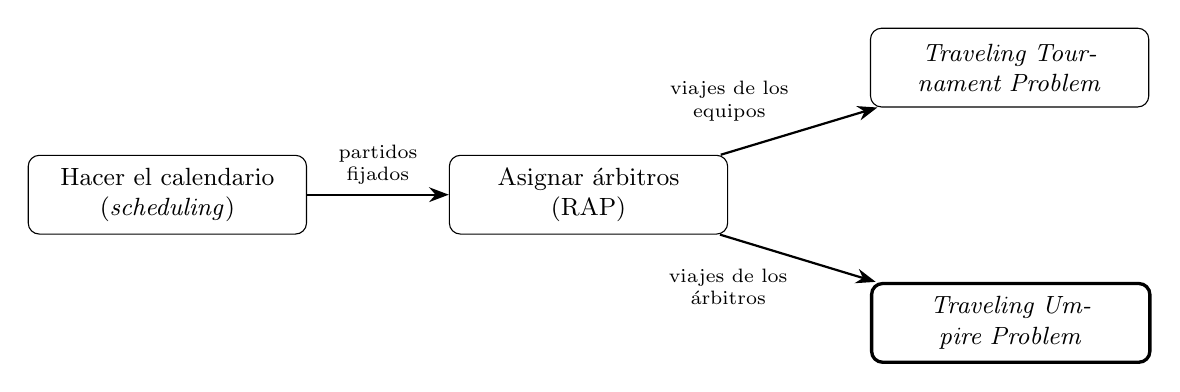
\begin{tikzpicture}[
  node distance=8mm,
  caja/.style={rectangle, rounded corners, draw, align=center, minimum height=10mm, text width=33mm, font=\small},
  cajafuerte/.style={rectangle, rounded corners, draw, very thick, align=center, minimum height=10mm, text width=33mm, font=\small},
  flecha/.style={-{Stealth[length=2.5mm]}, thick}
]
\node[caja] (cal) {Hacer el calendario\\(\emph{scheduling})};
\node[caja, right=18mm of cal] (rap) {Asignar árbitros\\(RAP)};
\node[caja, above right=6mm and 18mm of rap] (ttp) {\emph{Traveling Tournament Problem}};
\node[cajafuerte, below right=6mm and 18mm of rap] (tup) {\emph{Traveling Umpire Problem}};
\draw[flecha] (cal) -- node[above, font=\scriptsize, align=center] {partidos\\fijados} (rap);
\draw[flecha] (rap) -- node[above left, font=\scriptsize, align=center] {viajes de los\\equipos} (ttp);
\draw[flecha] (rap) -- node[below left, font=\scriptsize, align=center] {viajes de los\\árbitros} (tup);
\end{tikzpicture}
\caption{Dónde encaja la asignación de árbitros dentro de la programación deportiva: primero se fija el calendario, después se asignan los árbitros y, cuando los desplazamientos importan, el problema se acerca al \emph{Traveling Tournament Problem} y al \emph{Traveling Umpire Problem}.}
\label{fig:familia}
\fuente{elaboración propia.}
\end{figure}

Dos de esos problemas parecidos merecen una mención aparte, porque comparten con el caso asturiano la preocupación por los viajes. El \emph{Traveling Tournament Problem} (TTP), propuesto por \citeA{easton2001ttp}, busca un calendario de liga que haga que los equipos recorran la menor distancia posible; es tan difícil que \citeA{thielen2011complexity} demostraron que es NP-duro, y se ha usado mucho como banco de pruebas para comparar algoritmos. Aún más cercano a la asignación de árbitros es el \emph{Traveling Umpire Problem} (TUP), que plantearon \citeA{yildiz2007benders} a partir de un caso real: aquí se trata de decidir qué cuadrilla arbitra cada partido gastando los mínimos kilómetros, con la condición de que cada árbitro visite todas las sedes y no repita demasiado. La idea de tratar la asignación de árbitros de béisbol con ayuda del ordenador viene de antes: ya \citeA{evans1988umpire} montó en los años ochenta un sistema para asignar las cuadrillas de la liga americana, y el TUP recogió después ese problema y le dio forma matemática. Para resolverlo, \citeA{trick2011benders} propusieron una búsqueda guiada por cortes de Benders que todavía hoy es una de las técnicas de referencia. Como reducir los desplazamientos es justo uno de los objetivos de mi trabajo, el TUP es una referencia especialmente útil, y vuelvo sobre las técnicas con las que se ha atacado en las secciones siguientes.

\section{Métodos exactos basados en modelos matemáticos}
\label{sec:exactos}

El primer grupo de técnicas que se ha aplicado al RAP son los métodos exactos. La idea es escribir el problema como un modelo matemático y resolverlo hasta encontrar la mejor solución posible (o demostrar que no hay otra mejor). Su gran ventaja es que dan esa garantía; su problema es el tiempo, que crece muy deprisa según aumenta el tamaño del caso. Dentro de este grupo distingo dos ramas: la programación lineal entera y la programación con restricciones.

\subsection{Programación lineal entera}

La programación lineal entera (\emph{Integer Linear Programming}, ILP) describe el problema con variables que solo valen 0 o 1 —por ejemplo, «el árbitro $i$ dirige el partido $j$» vale 1 si lo hace y 0 si no—, sujetas a un conjunto de restricciones lineales, y se resuelve con la técnica de ramificación y acotación, que se remonta a \citeA{land1960branch}. Es, con diferencia, el método más usado para asignar árbitros en ligas profesionales. \citeA{yavuz2008fair} escribieron la asignación justa de la liga turca como un modelo entero que resolvían semana a semana. \citeA{linfati2012referee} abordó la Serie A italiana de voleibol —el caso más parecido al mío— con un modelo de programación lineal entera al que añadió una descomposición basada en grafos para que calculara más rápido, y lo probó con datos reales del campeonato. \citeA{mancini2014fair} hicieron algo parecido para el fútbol italiano, centrándose en la equidad. Y el grupo de Linfati amplió después su modelo a un calendario deportivo flexible que tiene en cuenta de forma explícita el coste de los viajes \cite{linfati2019flexible}.

Esta misma línea ha dado muy buenos resultados al programar ligas enteras en Latinoamérica: \citeA{duran2007chile} programaron la liga chilena de fútbol con programación entera, y \citeA{recalde2013ecuadorian} hicieron lo mismo con la liga profesional de Ecuador, y en ambos casos los modelos se usaron de verdad. La lección es clara: cuando el problema se puede escribir de forma limpia y el caso no es enorme, los métodos exactos dan soluciones óptimas y fáciles de explicar y de revisar, algo que las federaciones agradecen.

\subsection{Programación con restricciones y el solver CP-SAT}

La programación con restricciones (\emph{Constraint Programming}, CP) es la segunda rama. En lugar de empezar por una función objetivo lineal, describe el problema con variables y reglas lógicas, y busca la solución combinando dos cosas: ir descartando opciones imposibles (propagación) y explorar las que quedan; el libro de referencia es el manual de \citeA{rossi2006cp}. La CP va muy bien con las reglas «duras» y combinatorias —horarios incompatibles, conflictos de interés, asignaciones que se excluyen— que en un modelo puramente lineal son incómodas de escribir.

En los últimos años la línea entre CP y programación entera se ha ido borrando gracias a los solvers que mezclan ambas. El más conocido es CP-SAT, el motor de programación con restricciones de OR-Tools, la biblioteca libre de Google \cite{ortools}. CP-SAT resuelve problemas con variables enteras apoyándose en un motor SAT mediante una técnica llamada \emph{lazy clause generation}, propuesta por \citeA{stuckey2010lazy}, y la combina con el método símplex para la parte lineal y con varias estrategias de búsqueda que corren en paralelo \cite{cpsat}. Gracias a eso puede manejar a la vez reglas lógicas complicadas y objetivos numéricos como reducir los kilómetros, que es justo lo que pide el caso asturiano. Por eso he elegido CP-SAT como núcleo exacto del sistema, una decisión que retomo en el Capítulo~\ref{cap:desarrollo}. Vale la pena señalar que la idea de guiar una búsqueda exacta no es ajena al deporte: \citeA{yildiz2007benders} resolvieron el TUP con cortes de Benders que dirigen la búsqueda, una idea muy parecida a la que usan los solvers modernos.

La Tabla~\ref{tab:exacto_vs_aprox} compara, a grandes rasgos, las ventajas y los límites de los métodos exactos frente a los aproximados que veré a continuación.

\begin{table}[ht]
\centering
\caption{Comparación general entre los métodos exactos y los aproximados aplicados a la asignación de árbitros, según la garantía de optimalidad, la capacidad de crecer con el tamaño del problema y la facilidad para añadir reglas nuevas.}
\label{tab:exacto_vs_aprox}
\begin{tabular}{@{}p{3.2cm}p{4.6cm}p{4.6cm}@{}}
\toprule
{\bf Criterio} & {\bf Métodos exactos (ILP / CP)} & {\bf Métodos aproximados (heurísticas / metaheurísticas)} \\
\midrule
Optimalidad & Garantizada, o con una cota de calidad demostrable & Sin garantía, pero buenas soluciones \\
Tamaño que admiten & Limitado: el tiempo crece muy rápido & Alto: soluciones útiles en tiempo acotado \\
Reglas complicadas & Cómodas en CP, más rígidas en ILP & Muy fáciles de añadir \\
Esfuerzo de modelado & Alto y formal & Medio, centrado en diseñar el algoritmo \\
Reproducibilidad & Total & Sujeta a algo de azar controlado \\
\bottomrule
\end{tabular}
\fuente{elaboración propia a partir de \citeA{kendall2010scheduling} y \citeA{ribeiro2012sports}.}
\end{table}

\section{Métodos aproximados: heurísticas y metaheurísticas}
\label{sec:aproximados}

Cuando el problema crece —cientos de partidos y decenas de árbitros cada fin de semana, como pasa en Asturias— los métodos exactos pueden tardar demasiado en cerrar la solución óptima. Ahí entran las heurísticas y las metaheurísticas, que renuncian a esa garantía a cambio de dar soluciones buenas en poco tiempo. No son técnicas de segunda fila: como recuerdan \citeA{kendall2010scheduling}, la mayor parte de la literatura reciente sobre programación deportiva se apoya en ellas. La Figura~\ref{fig:taxonomia} ordena en un mapa las familias que describo a continuación.

\begin{figure}[ht]
\centering
\resizebox{\textwidth}{!}{%
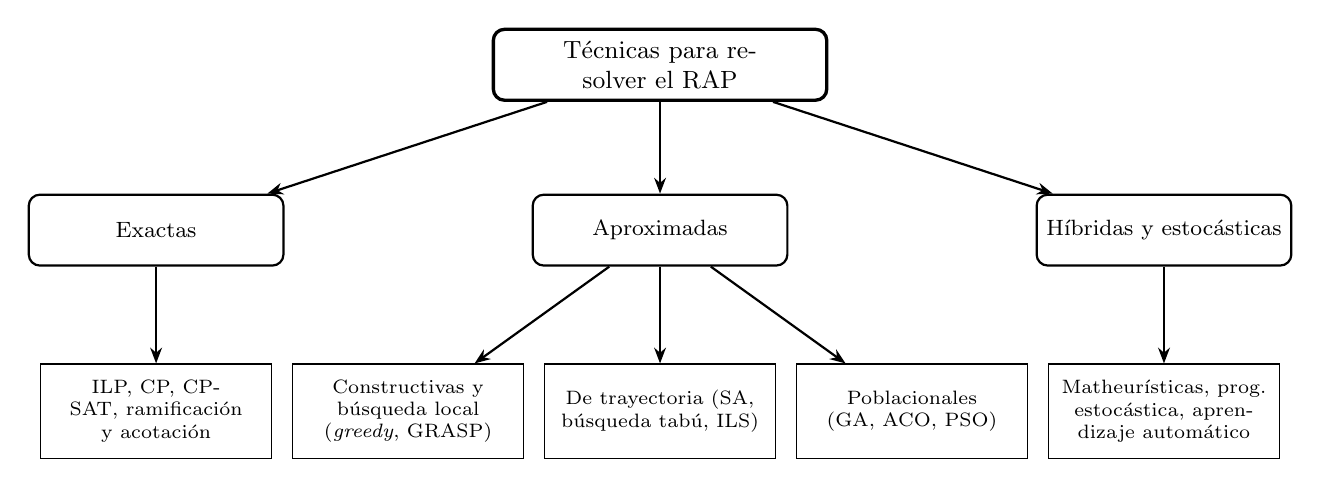
\begin{tikzpicture}[
  raiz/.style={rectangle, rounded corners, draw, very thick, align=center, font=\small, text width=40mm, minimum height=9mm},
  cat/.style={rectangle, rounded corners, draw, thick, align=center, font=\footnotesize, text width=30mm, minimum height=9mm},
  hoja/.style={rectangle, draw, align=center, font=\scriptsize, text width=27mm, minimum height=12mm},
  lin/.style={-{Stealth[length=2mm]}, thick}
]
% raíz
\node[raiz] (raiz) at (0,0) {Técnicas para resolver el RAP};
% categorías (nivel intermedio), bien separadas
\node[cat] (ex) at (-6.4,-2.1) {Exactas};
\node[cat] (ap) at (0,-2.1) {Aproximadas};
\node[cat] (hi) at (6.4,-2.1) {Híbridas y estocásticas};
% hojas
\node[hoja] (exh) at (-6.4,-4.4) {ILP, CP, CP-SAT, ramificación y acotación};
\node[hoja] (ap1) at (-3.2,-4.4) {Constructivas y búsqueda local (\emph{greedy}, GRASP)};
\node[hoja] (ap2) at (0,-4.4) {De trayectoria (SA, búsqueda tabú, ILS)};
\node[hoja] (ap3) at (3.2,-4.4) {Poblacionales (GA, ACO, PSO)};
\node[hoja] (hih) at (6.4,-4.4) {Matheurísticas, prog.\ estocástica, aprendizaje automático};
% aristas raíz -> categorías
\draw[lin] (raiz) -- (ex);
\draw[lin] (raiz) -- (ap);
\draw[lin] (raiz) -- (hi);
% aristas categorías -> hojas
\draw[lin] (ex) -- (exh);
\draw[lin] (ap) -- (ap1);
\draw[lin] (ap) -- (ap2);
\draw[lin] (ap) -- (ap3);
\draw[lin] (hi) -- (hih);
\end{tikzpicture}%
}
\caption{Mapa de las principales técnicas usadas para resolver el problema de asignación de árbitros y otros problemas de programación deportiva, agrupadas en exactas, aproximadas e híbridas.}
\label{fig:taxonomia}
\fuente{elaboración propia.}
\end{figure}

\subsection{Heurísticas constructivas y búsqueda local}

Las heurísticas constructivas construyen una solución desde cero, tomando decisiones golosas una detrás de otra: en cada paso eligen la asignación que parece mejor en ese momento. Son rápidas y dan un punto de partida razonable, aunque casi nunca el óptimo. Su complemento natural es la búsqueda local, que parte de una solución completa y la va mejorando con cambios pequeños —mover un árbitro de un partido a otro, intercambiar dos asignaciones— mientras eso reduzca el coste. Un esquema muy conocido que junta las dos ideas es GRASP (\emph{Greedy Randomized Adaptive Search Procedure}), que propusieron \citeA{feo1995grasp}: añade un poco de azar a la fase constructiva y luego pule cada solución con búsqueda local.

Esta pareja —construir y luego mejorar— es justo lo que sostiene los dos trabajos más importantes sobre el RAP. \citeA{duarte2007referee} propusieron una heurística de tres fases: una construcción golosa, una fase para arreglar lo que quede mal y una mejora final con búsqueda local; la probaron con casos realistas de hasta cientos de partidos. \citeA{yavuz2008fair}, por su parte, juntaron una construcción con una búsqueda local que resolvía el caso de la liga turca en un segundo y con muy buena calidad. Este mismo esquema es el que usa el sistema de este Trabajo, donde una fase golosa prepara el terreno para el solver exacto y una búsqueda local pule el resultado al final.

\subsection{Metaheurísticas de trayectoria}

Las metaheurísticas son estrategias de más alto nivel que coordinan heurísticas sencillas para no quedarse atascadas en óptimos locales, que es donde la búsqueda local a secas se suele parar. Las de trayectoria trabajan sobre una sola solución que van transformando. El recocido simulado (\emph{Simulated Annealing}, SA), que propusieron \citeA{kirkpatrick1983sa} inspirándose en cómo se enfrían los metales, acepta de vez en cuando cambios que empeoran la solución para no quedarse encerrado, con una probabilidad que va bajando con el tiempo. La búsqueda tabú, que formalizó \citeA{glover1986tabu}, hace otra cosa: prohíbe durante un rato deshacer los últimos movimientos —los marca como «tabú»— para obligar a explorar zonas nuevas. Y la búsqueda local iterada (\emph{Iterated Local Search}, ILS), descrita por \citeA{lourenco2003ils}, alterna búsquedas locales con pequeñas sacudidas que sacan a la solución de su óptimo local para volver a empezar desde un punto cercano pero distinto.

Estas tres técnicas han funcionado bien en problemas muy cercanos al RAP. Para el \emph{Traveling Tournament Problem}, \citeA{lim2006sahc} combinaron recocido simulado con \emph{hill-climbing}, \citeA{anagnostopoulos2006sa} hicieron un recocido simulado con movimientos a medida que mejoró las mejores soluciones conocidas hasta entonces, y \citeA{digaspero2007tabu} lograron buenos resultados con una búsqueda tabú. La ILS, por su lado, fue la pieza con la que \citeA{duarte2007hybridils} llevaron su heurística del RAP un paso más allá, como cuento en la Sección~\ref{sec:hibridos}.

\subsection{Metaheurísticas poblacionales}

A diferencia de las anteriores, las metaheurísticas poblacionales no trabajan con una sola solución, sino con un grupo de ellas que va evolucionando a la vez. Los algoritmos genéticos (\emph{Genetic Algorithms}, GA), cuyas bases puso \citeA{holland1975adaptation} y que popularizó \citeA{goldberg1989genetic}, imitan la selección natural: cada solución es como un «cromosoma» y se generan nuevas combinándolas (cruce) y cambiándolas un poco (mutación), guardando siempre las mejores de cada generación. La optimización por colonia de hormigas (\emph{Ant Colony Optimization}, ACO), que introdujo \citeA{dorigo1996ant}, se inspira en cómo las hormigas encuentran caminos cortos dejando rastros de feromonas. Y la optimización por enjambre de partículas (\emph{Particle Swarm Optimization}, PSO), de \citeA{kennedy1995pso}, trata las soluciones como partículas que se mueven por el espacio guiándose por su propia experiencia y por la del grupo.

De todas ellas, la que más se ha usado en la asignación de árbitros es el algoritmo genético. \citeA{trick2012crossover} diseñaron para el TUP un operador de cruce mejorado que superaba a las soluciones del recocido simulado y —lo más relevante para mi caso— \citeA{meng2014volleyball} usaron un algoritmo genético para asignar árbitros a sus horarios preferidos en torneos de voleibol, dejando la programación entera solo para decidir cuántos equipos había en cada división. Es uno de los pocos antecedentes que juntan voleibol y metaheurísticas, así que lo tomo como punto de comparación.

La Tabla~\ref{tab:metaheuristicas} reúne las principales metaheurísticas que he mencionado, con el artículo donde se propusieron, su idea central, sus ventajas e inconvenientes y un ejemplo de uso en programación deportiva. En cada caso he puesto la referencia del trabajo original, para dar crédito a quienes introdujeron cada idea.

\begin{table}[ht]
\centering
\footnotesize
\caption{Principales metaheurísticas usadas en la asignación de árbitros y en la programación deportiva, con el artículo original donde se propusieron, su idea básica, sus ventajas e inconvenientes y un ejemplo de uso.}
\label{tab:metaheuristicas}
\begin{tabular}{@{}p{2.3cm}p{1.9cm}p{2.6cm}p{3.0cm}p{2.4cm}@{}}
\toprule
{\bf Técnica} & {\bf Origen} & {\bf Idea central} & {\bf Ventajas / inconvenientes} & {\bf Ejemplo de uso} \\
\midrule
Recocido simulado (SA) & \citeA{kirkpatrick1983sa} & Acepta empeoramientos con probabilidad cada vez menor & Simple y eficaz / hay que ajustar bien el enfriamiento & TTP \cite{anagnostopoulos2006sa} \\
Búsqueda tabú & \citeA{glover1986tabu} & Prohíbe deshacer los movimientos recientes & Explora bien / hay que ajustar la memoria tabú & TTP \cite{digaspero2007tabu} \\
Búsqueda local iterada (ILS) & \citeA{lourenco2003ils} & Sacude la solución y vuelve a optimizar & Sencilla y robusta / depende de la sacudida & RAP \cite{duarte2007hybridils} \\
Algoritmo genético (GA) & \citeA{holland1975adaptation} & Evoluciona un grupo de soluciones con cruce y mutación & Muy flexible / converge despacio y tiene muchos parámetros & TUP \cite{trick2012crossover}; voleibol \cite{meng2014volleyball} \\
Colonia de hormigas (ACO) & \citeA{dorigo1996ant} & Refuerza los caminos buenos con feromonas & Buena en rutas / cálculo costoso & Calendarios deportivos \\
Enjambre de partículas (PSO) & \citeA{kennedy1995pso} & Partículas guiadas por su mejor posición y la del grupo & Converge rápido / puede estancarse pronto & Optimización combinatoria en general \\
\bottomrule
\end{tabular}
\fuente{elaboración propia a partir de las fuentes citadas.}
\end{table}

\section{Métodos híbridos, incertidumbre y aprendizaje automático}
\label{sec:hibridos}

La tendencia que mejor ha funcionado en los últimos años no es elegir entre métodos exactos y aproximados, sino combinarlos. Estas \emph{matheurísticas} aprovechan la calidad de los modelos matemáticos en problemas pequeños y la rapidez de las metaheurísticas para coordinarlo todo. El mejor ejemplo en nuestro terreno es el trabajo de \citeA{duarte2007hybridils}, que juntaron una búsqueda local iterada con un modelo entero por dentro (ILS$+$MIP) para resolver el RAP: la metaheurística dirige la exploración y, en cada paso, un modelo entero resuelve de forma óptima la reasignación dentro de una zona pequeña. Los mismos autores estudiaron después versiones con varios objetivos a la vez, tanto exactas como aproximadas \cite{duarte2008multiobjective}. En el TUP pasa lo mismo: \citeA{yildiz2007benders} guían una búsqueda amplia con cortes de Benders, y \citeA{toffolo2016tup} consiguen cotas muy ajustadas con un esquema de ramificación y acotación basado en descomposición. El sistema que presento en este Trabajo está de lleno en esta corriente híbrida, ya que encadena una heurística golosa, el solver exacto CP-SAT y una búsqueda local.

Una segunda línea más reciente tiene en cuenta la incertidumbre de forma explícita. En la realidad no se sabe con total seguridad ni cómo rendirá un árbitro ni lo difícil que será un partido cuando toca planificar, y la programación estocástica permite reflejar esa variabilidad. \citeA{canakoglu2026stochastic} plantearon precisamente una asignación de árbitros con incertidumbre mediante un modelo por etapas que decide, por un lado, qué árbitros entran cada jornada pensando a largo plazo y, por otro, a qué partidos van según la dificultad que se espera; como resolver el modelo completo es demasiado costoso, usan una aproximación basada en \emph{sample average approximation}.

Por último, el aprendizaje automático empieza a aparecer en este terreno, aunque con mucho menos recorrido que la optimización clásica. Su papel más natural no es sustituir al optimizador, sino darle datos: estimar la disponibilidad o el rendimiento de los árbitros, predecir lo difícil que será un partido o aprender las preferencias de quien hoy hace las asignaciones a mano para meterlas como pesos en el objetivo. Es una vía todavía muy poco explorada en la asignación de árbitros, así que la dejo como línea de trabajo futuro en el Capítulo~\ref{cap:conclusiones}. Conviene además recordar que el RAP se parece mucho al problema más general de organizar turnos de personal, cuya revisión clásica de \citeA{ernst2004rostering} sigue siendo una buena guía de técnicas que se pueden trasladar.

\section{Resumen comparativo y posición de este Trabajo}
\label{sec:sintesis}

En resumen, la literatura ha tratado la asignación de árbitros como un problema de optimización con muchas reglas y, muchas veces, con varios objetivos que chocan entre sí. La Tabla~\ref{tab:panoramica} reúne los trabajos más representativos, ordenados por la técnica principal que usan, para ver de un vistazo qué se ha hecho, en qué deporte y con qué objetivo.

\begin{table}[ht]
\centering
\footnotesize
\caption{Resumen comparativo de trabajos representativos sobre asignación de árbitros y problemas de programación deportiva cercanos, según la técnica principal, el deporte o liga, el objetivo y el tamaño de los casos resueltos.}
\label{tab:panoramica}
\begin{tabular}{@{}p{3.2cm}p{2.9cm}p{2.4cm}p{3.1cm}@{}}
\toprule
{\bf Trabajo} & {\bf Técnica principal} & {\bf Deporte / liga} & {\bf Objetivo principal} \\
\midrule
\citeA{duarte2007referee} & Heurística de tres fases & Fútbol amateur & Que la solución sea válida y con pocos viajes \\
\citeA{duarte2007hybridils} & ILS $+$ MIP (híbrido) & Genérico (RAP) & Calidad y capacidad de crecer \\
\citeA{yavuz2008fair} & ILP $+$ búsqueda local & Fútbol (Turquía) & Equidad \\
\citeA{linfati2012referee} & ILP $+$ grafos & Voleibol (Italia) & Coste y carga \\
\citeA{mancini2014fair} & ILP & Fútbol (Italia) & Equidad \\
\citeA{trick2012mlb} & SA / GA (TUP) & Béisbol (MLB) & Reducir viajes \\
\citeA{meng2014volleyball} & GA $+$ ILP & Voleibol & Horarios preferidos \\
\citeA{canakoglu2026stochastic} & Prog.\ estocástica & Genérico (RAP) & Aguantar la incertidumbre \\
\midrule
{\bf Este Trabajo} & {\bf \emph{Greedy} $+$ CP-SAT $+$ b.\ local} & {\bf Voleibol (Asturias)} & {\bf Reducir viajes y repartir con equidad} \\
\bottomrule
\end{tabular}
\fuente{elaboración propia a partir de las fuentes citadas.}
\end{table}

De este resumen saco tres conclusiones que guían el diseño del sistema. La primera es que el enfoque híbrido es el que mejor encaja en un problema que tiene reglas duras y, a la vez, un objetivo numérico: por eso uso la combinación de una heurística golosa, el solver exacto CP-SAT \cite{cpsat} y una búsqueda local, en la línea del esquema de tres fases de \citeA{duarte2007referee} y de la matheurística ILS$+$MIP de \citeA{duarte2007hybridils}. La segunda es que reducir los desplazamientos, que es lo importante en Asturias, conecta directamente con la familia del \emph{Traveling Umpire Problem} de \citeA{yildiz2007benders}, lo que justifica ponerlo en el centro del objetivo. Y la tercera es que la equidad en el reparto, que \citeA{yavuz2008fair} convirtieron en un principio básico, tiene que formar parte del modelo desde el principio y no añadirse como un parche al final.

También merece la pena dejar claro qué he descartado y por qué, porque eso también forma parte del trabajo. Un enfoque puramente exacto con ILP, como el de \citeA{linfati2012referee}, sería muy elegante pero costaría mucho escalarlo a los más de cien partidos por semana de la federación asturiana sin que los tiempos se disparen, y además resulta incómodo para escribir reglas lógicas como el coche compartido o los conflictos de interés; CP-SAT maneja mejor esa parte. Una metaheurística poblacional pura, como el algoritmo genético de \citeA{meng2014volleyball}, daría flexibilidad pero perdería la garantía de calidad que sí ofrece el solver exacto en los casos de tamaño medio que aparecen en la práctica. La opción híbrida que he elegido busca precisamente quedarse con lo mejor de cada lado. En el Capítulo~\ref{cap:desarrollo} concreto esta decisión en un modelo y en una implementación, y en el de conclusiones la comparo con el proceso manual que hoy usa la FVBPA.

% NOTA: aquí encaja muy bien una figura adaptada de alguno de los trabajos citados
% (p. ej., el esquema de las tres fases de Duarte et al., 2007, o un ejemplo de
% asignación de Linfati, 2012). Recuerda incluir la atribución bajo el caption,
% del tipo \fuente{adaptado de \citeA{duarte2007referee}.}, y NO reproducir la
% figura original tal cual, sino redibujarla con tus propios datos o esquema.
% \begin{figure}[ht]
% \centering
% \includegraphics[width=0.8\textwidth]{tres_fases}
% \caption{Esquema de las tres fases del enfoque adoptado: construcción golosa, optimización exacta y mejora por búsqueda local.}
% \label{fig:tresfases}
% \fuente{elaboración propia, adaptado de \citeA{duarte2007referee}.}
% \end{figure}

%==================================================
\chapter{Identificación de requisitos}

Aquí defino qué tiene que cumplir el sistema para que sea funcional, eficiente y adaptable al entorno real de la federación. Primero van los requisitos funcionales —gestión de datos, generación de asignaciones y visualización de resultados— y luego los no funcionales, que tocan rendimiento, escalabilidad, usabilidad, mantenibilidad y fiabilidad. Todos ellos servirán de base para el diseño y la implementación.

\section{Requisitos funcionales}

Estos son los requisitos que debe satisfacer el sistema para responder a lo que pide la federación.

\begin{itemize}
\item {\bf RF1: Gestión de datos de entrada.} El sistema debe aceptar como entrada los siguientes conjuntos de datos:
    \begin{itemize}
    \item {\bf RF1.1: Árbitros.} Datos completos de cada árbitro (nombre, apellidos, nivel y domicilio o ubicación de referencia).
    \item {\bf RF1.2: Disponibilidad horaria.} Para cada árbitro y día, la disponibilidad por franjas (9:00–12:00, 12:00–15:00, 15:00–18:00, 18:00–22:00), indicando si está disponible con transporte, sin transporte o no disponible.
    \item {\bf RF1.3: Partidos.} Datos de cada partido programado (sede, fecha, hora, equipo local, visitante, categoría, nivel mínimo de árbitro y número mínimo de árbitros a asignar).
    \item {\bf RF1.4:} De forma opcional, poder actualizar estos datos —añadir o quitar árbitros, partidos u horarios— antes de lanzar la asignación.
    \end{itemize}
\item {\bf RF2: Algoritmo de asignación inteligente.} El sistema debe incorporar un algoritmo de optimización basado en IA que genere automáticamente las asignaciones cumpliendo todas las restricciones. En concreto:
    \begin{itemize}
    \item {\bf RF2.1:} Respetar la disponibilidad de cada árbitro. Nunca asignarlo a una franja marcada como no disponible; si está disponible sin transporte, solo darle partidos en sedes locales o cercanas.
    \item {\bf RF2.2:} Garantizar que cada partido recibe el número mínimo de árbitros y que cada uno cumple el nivel mínimo de la categoría.
    \item {\bf RF2.3: Optimización geográfica.} Minimizar la distancia o el tiempo de viaje. Si un árbitro dirige varios partidos en un día, agrupárselos en sedes próximas o consecutivas.
    \item {\bf RF2.4: Conflictos de interés.} Un árbitro no debe acabar en un partido en el que él o un familiar directo juega. Esta comprobación se hace automáticamente.
    \item {\bf RF2.5: Equidad y balance.} Repartir los partidos de forma equilibrada y evitar emparejar una y otra vez al mismo árbitro con el mismo equipo.
    \item {\bf RF2.6: Heurísticas y aprendizaje automático.} Como el problema es NP-completo, el algoritmo puede combinar optimización matemática (programación entera o por restricciones) con heurísticas y aprendizaje automático para dar buenas soluciones en tiempo razonable.
    \end{itemize}
\item {\bf RF3: Salida y visualización de resultados.} El sistema debe presentar los resultados de forma accesible:
    \begin{itemize}
    \item {\bf RF3.1: Interfaz gráfica sencilla.} Un calendario interactivo que muestre los partidos con sus árbitros y permita revisarlos.
    \item {\bf RF3.2: Exportación.} Poder exportar la asignación final, al menos a Excel (XLS/XLSX) y PDF, para usarla fuera de la aplicación.
    \item {\bf RF3.3:} Posibilidad de reajustar o relanzar la asignación tras cambios pequeños, como una sustitución de última hora.
    \end{itemize}
\end{itemize}

En síntesis, lo funcional gira en torno a tres cosas: gestionar los datos de árbitros y partidos, generar las asignaciones con un algoritmo inteligente y presentar o exportar los resultados.

\section{Requisitos no funcionales}

Además, el sistema debe cumplir ciertos criterios de calidad:

\begin{itemize}
\item {\bf RNF1: Rendimiento y escalabilidad.} Debe procesar escenarios de tamaño real —cientos de partidos semanales y decenas de árbitros— en un tiempo razonable. Dado que el problema es NP-completo, se espera que las heurísticas den soluciones viables sin que los cálculos se eternicen.
    \begin{itemize}
    \item {\bf RNF1.1: Escalabilidad.} Al crecer el número de árbitros o partidos, el tiempo de cómputo debe aumentar de forma controlada, y el sistema debe funcionar para ligas de distinto tamaño sin hardware especializado.
    \end{itemize}
\item {\bf RNF2: Calidad de la solución.} Aunque no siempre se alcance el óptimo teórico, las asignaciones deben cumplir las restricciones duras (disponibilidad, nivel, conflictos) y acercarse al mínimo de desplazamientos. Con las mismas entradas, los resultados deben ser consistentes, salvo por una aleatoriedad controlada.
\item {\bf RNF3: Usabilidad.} La interfaz debe ser intuitiva y centrada en el algoritmo. Aunque la prioridad es la robustez del cálculo, conviene cuidar los tiempos de carga y dar mensajes de error claros cuando falten datos o haya incompatibilidades.
\item {\bf RNF4: Interoperabilidad.} Usar formatos abiertos (CSV/Excel para entrada, PDF/Excel para salida) para integrarse con lo que ya usa la federación, sin obligar a software propietario.
\item {\bf RNF5: Mantenibilidad y documentación.} El sistema —código y manual— debe estar bien documentado, y el algoritmo debe ser modular, de modo que añadir reglas o mejorar heurísticas no obligue a rehacerlo todo.
\item {\bf RNF6: Fiabilidad.} Debe gestionar errores en los datos (valores que faltan o incoherentes) de forma controlada, avisar al usuario y garantizar la integridad de entradas y salidas, sin perder asignaciones al exportar.
\end{itemize}

Con estos requisitos no funcionales el sistema no solo cumple su cometido, sino que resulta eficiente, robusto y manejable en el día a día de la FVBPA.

%==================================================
\chapter{Objetivos}

En este capítulo fijo las metas del trabajo, generales y específicas, que guían el desarrollo del sistema de asignación.

\noindent{\bf Objetivo general:} diseñar, implementar y validar un sistema inteligente, basado en inteligencia artificial, para la asignación arbitral en las competiciones de voleibol del Principado de Asturias, optimizando los desplazamientos y mejorando la eficiencia y la equidad del proceso de designación.

\vspace{0.3cm}
\noindent{\bf Objetivos específicos:}

\begin{itemize}
\item {\bf Analizar el estado actual.} Estudiar y describir el método manual que usa la federación, identificando sus puntos débiles: errores, carga de trabajo y tiempos de cálculo.
\item {\bf Modelar el problema.} Formalizar la asignación como una optimización combinatoria con restricciones (disponibilidad, niveles, geolocalización, conflictos, equidad), definiendo variables de decisión, restricciones y función objetivo.
\item {\bf Desarrollar el algoritmo.} Integrar optimización matemática (programación entera o por restricciones) con heurísticas y/o aprendizaje automático, y ajustarlo para que genere asignaciones viables que minimicen viajes y respeten las reglas.
\item {\bf Implementar el prototipo.} Programar el sistema en una plataforma adecuada con la interfaz mínima necesaria, asegurando que lee bien los datos de árbitros y partidos y que la salida es visualizable y exportable.
\item {\bf Validar y evaluar.} Probarlo con datos reales y simulados de la federación, comparándolo con el método manual en calidad y tiempo. Medir indicadores como el kilometraje total, el cumplimiento de restricciones o la equidad del reparto.
\item {\bf Optimizar y ajustar.} Mejorar el algoritmo de forma iterativa —calibrar heurísticas, probar nuevas técnicas— para ganar calidad o reducir tiempos.
\item {\bf Documentar y presentar.} Redactar la memoria final con los antecedentes, el diseño del modelo, la implementación, los resultados y las conclusiones sobre la mejora lograda.
\end{itemize}

Con esto se cubren todas las fases del trabajo, desde el análisis y la revisión bibliográfica hasta el desarrollo técnico y la evaluación práctica.

% NOTA: figura "Flujo de desarrollo de TFM / Objetivos específicos" omitida por ahora.

%==================================================
\chapter{Desarrollo del trabajo}
\label{cap:desarrollo}

Este es el capítulo donde de verdad se ve cómo está hecho el sistema. En los anteriores he explicado qué problema quiero resolver, qué se ha hecho antes y qué condiciones tiene que cumplir la solución; aquí cuento cómo lo he construido, desde la arquitectura general hasta la última restricción del algoritmo. Lo he organizado de fuera hacia dentro: primero la foto de conjunto y la arquitectura (Sección~\ref{sec:arquitectura}), después de dónde salen los datos y cómo los guardo (Sección~\ref{sec:datos}), luego un recorrido por la interfaz para que se entienda qué hace la aplicación de cara al usuario (Sección~\ref{sec:interfaz}) y, a partir de ahí, ya entro en el corazón del trabajo: el modelado formal del problema (Sección~\ref{sec:modelo}), la preparación de la instancia (Sección~\ref{sec:instancia}), las tres fases del algoritmo de asignación (Sección~\ref{sec:algoritmo}), el cálculo de los desplazamientos con coche compartido (Sección~\ref{sec:coche}) y, por último, los resultados sobre datos reales de la federación (Sección~\ref{sec:resultados}).

Todo el código que enseño a trozos a lo largo del capítulo está sacado del proyecto, que se llama \emph{RefMe}; en el Anexo~B aparecen las funciones completas.

\section{Visión general y arquitectura}
\label{sec:arquitectura}

Lo primero que decidí fue qué forma tendría el producto. Tenía claro que no quería un script suelto que se lanzara desde la terminal: la federación necesita meter datos, revisarlos, lanzar la asignación y ver el resultado de una forma cómoda, así que monté una aplicación web de toda la vida, con un servidor por detrás y una interfaz por delante. La idea era que cualquiera de la federación pudiera usarla sin saber nada de programación.

La arquitectura es deliberadamente sencilla, en parte por una de las limitaciones que me había puesto en el Capítulo~3: nada de tecnologías caras ni de infraestructura difícil de mantener. El sistema tiene tres piezas:

\begin{itemize}
\item Un {\bf backend} en Python con \emph{FastAPI} \cite{fastapi}, que es el que expone una API REST y, sobre todo, contiene el motor de asignación. FastAPI me gustó porque es ligero, rápido de montar y genera la documentación de la API solo.
\item Una {\bf base de datos} SQLite gestionada con SQLAlchemy. SQLite es un fichero, no hace falta instalar ni administrar ningún servidor de base de datos, lo cual encaja perfectamente con la idea de mantenimiento barato.
\item Un {\bf frontend} web estático (HTML, CSS y JavaScript sin frameworks pesados) que el propio backend sirve. No quise meter React ni nada parecido para no complicar el despliegue: son unos cuantos ficheros que se cargan en el navegador y hablan con la API.
\end{itemize}

La Figura~\ref{fig:arquitectura} resume cómo encajan las piezas. El usuario trabaja contra el navegador, el navegador llama a la API del backend, y el backend habla con la base de datos y con el motor de asignación, que es donde está toda la chicha de este trabajo.

\begin{figure}[ht]
\centering
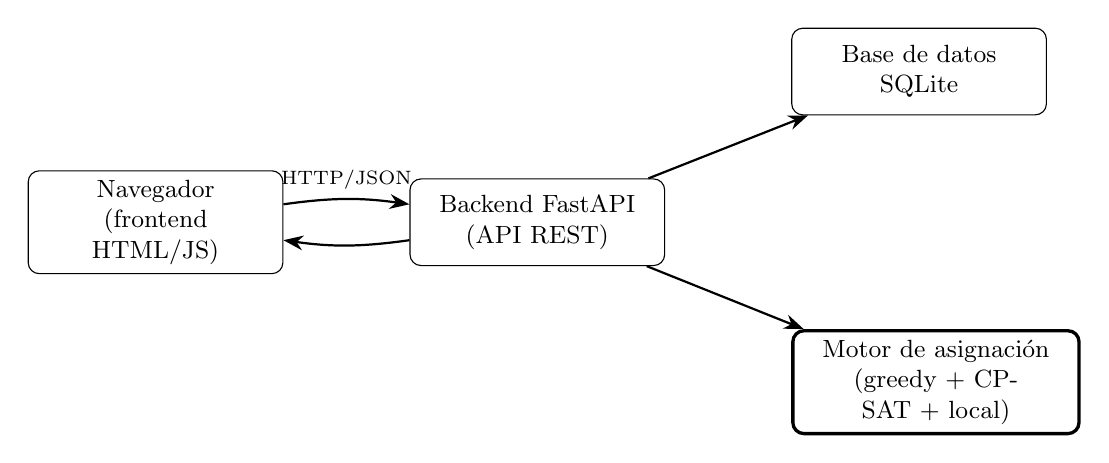
\begin{tikzpicture}[
  node distance=7mm,
  caja/.style={rectangle, rounded corners, draw, align=center, minimum height=11mm, text width=30mm, font=\small},
  cajam/.style={rectangle, rounded corners, draw, very thick, align=center, minimum height=11mm, text width=34mm, font=\small},
  flecha/.style={-{Stealth[length=2.5mm]}, thick}
]
\node[caja] (fe) {Navegador\\(frontend HTML/JS)};
\node[caja, right=16mm of fe] (api) {Backend FastAPI\\(API REST)};
\node[caja, above right=8mm and 16mm of api] (db) {Base de datos\\SQLite};
\node[cajam, below right=8mm and 16mm of api] (motor) {Motor de asignación\\(greedy + CP-SAT + local)};
\draw[flecha] (fe) to[bend left=8] node[above, font=\scriptsize]{HTTP/JSON} (api);
\draw[flecha] (api) to[bend left=8] (fe);
\draw[flecha] (api) -- (db);
\draw[flecha] (api) -- (motor);
\end{tikzpicture}
\caption{Arquitectura general del sistema: un frontend web que consume una API REST en FastAPI, la cual se apoya en una base de datos SQLite y en el motor de asignación.}
\label{fig:arquitectura}
\fuente{elaboración propia.}
\end{figure}

El backend está organizado por \emph{routers}, que son los grupos de endpoints de la API: hay uno para árbitros, otro para disponibilidad, otro para partidos, categorías, clubs, polideportivos, estadísticas y, el más importante, el de asignaciones. Por debajo de los routers están los modelos (las tablas de la base de datos) y un paquete \texttt{asignacion/} que contiene todo el algoritmo, separado en módulos. Esa separación no es por capricho: uno de los requisitos no funcionales (RNF5) pedía que el sistema fuera modular, de modo que tocar una restricción o cambiar una heurística no obligue a reescribir lo demás. Cada fase del algoritmo vive en su propio fichero y se puede cambiar de forma independiente.

Cuando el servidor arranca por primera vez, crea las tablas y carga los datos iniciales desde unos ficheros Excel que aporta la federación; esto lo cuento en la siguiente sección. A partir de ahí, todo funciona contra la base de datos.

\section{Origen y modelo de los datos}
\label{sec:datos}

Un sistema de optimización es tan bueno como los datos que le metes, así que esta parte me dio más trabajo del que parece. La federación no tiene una base de datos bonita de la que tirar: lo que tiene son hojas de Excel. En concreto manejé tres fuentes: la relación de licencias arbitrales (con el nombre, el código y el nivel de cada árbitro), un fichero de disponibilidad con su domicilio y las franjas en las que puede pitar, y el calendario de partidos con sus categorías. Además, la federación me pasó los polideportivos, los clubs y los equipos ya identificados con sus códigos.

El primer trabajo fue leer todo eso y volcarlo a una base de datos con una estructura coherente. El modelo de datos, que está en \texttt{models.py}, gira en torno a siete entidades principales. La Tabla~\ref{tab:entidades} las resume.

\begin{table}[ht]
\centering
\caption{Entidades principales del modelo de datos del sistema.}
\label{tab:entidades}
\begin{tabular}{@{}p{2.8cm}p{10.5cm}@{}}
\toprule
{\bf Entidad} & {\bf Qué guarda} \\
\midrule
Árbitro & Nombre, código de licencia, nivel arbitral, domicilio y coordenadas (latitud/longitud). \\
Nivel & Jerarquía de niveles arbitrales con un orden numérico, para comparar quién alcanza qué. \\
Categoría & Una competición y sus requisitos: qué roles exige (1.\textsuperscript{er} árbitro, 2.\textsuperscript{o}, anotador), el nivel mínimo de cada rol, el número mínimo de árbitros y la prioridad. \\
Equipo & Equipos de cada categoría (y su club). \\
Partido & Un encuentro del calendario: fecha, hora, categoría, equipos local y visitante, sede. \\
Disponibilidad & Para cada árbitro, fecha y franja horaria, si está disponible con transporte, sin transporte o no disponible. \\
Asignación & Un árbitro asignado a un partido en un rol concreto (manual o automática). \\
\bottomrule
\end{tabular}
\fuente{elaboración propia.}
\end{table}

Hay un detalle que me costó y que merece la pena contar: la geolocalización. Para optimizar los desplazamientos necesito saber dónde vive cada árbitro y dónde está cada polideportivo, pero en los Excel los domicilios vienen como direcciones de texto («Calle tal, número tal, Oviedo»). Lo que hice fue geocodificar esas direcciones, es decir, convertirlas en coordenadas (latitud y longitud), y guardar el resultado en una caché (\texttt{geocache.json}) para no repetir el trabajo. Cuando no consigo geocodificar una dirección exacta, caigo a una aproximación al centro del concejo, y marco ese árbitro como no geocodificado con precisión. Con los polideportivos fue más fácil porque la federación ya me los dio con coordenadas; el problema ahí era casar el nombre del campo que aparece en el calendario (texto libre, a veces con erratas) con el polideportivo correcto, lo que resuelvo normalizando los nombres y buscando coincidencias exactas o por subcadena. Con eso resuelvo 38 de las 39 sedes que aparecen en los datos.

Toda esta carga inicial está automatizada en el módulo \texttt{seed.py}, de modo que arrancar el sistema desde cero deja la base de datos lista para trabajar.

\section{La interfaz de usuario}
\label{sec:interfaz}

Antes de meterme en el algoritmo prefiero enseñar la aplicación por fuera, porque así se entiende mucho mejor para qué sirve cada cosa. La interfaz tiene una barra lateral fija con todas las secciones, agrupadas en tres bloques: «General» (el panel de control), «Datos» (árbitros, disponibilidad, clubs y categorías) y «Competición» (calendario y asignaciones). El estilo es limpio, con los colores de la federación, porque la idea era que diera sensación de herramienta seria y no de prototipo de laboratorio.

\subsection{Panel de control}

La pantalla de inicio es un panel de control (Figura~\ref{fig:dashboard}) que da una foto rápida del estado del sistema. Arriba hay cuatro contadores —árbitros, partidos, categorías y asignaciones— y debajo, a la izquierda, un resumen de cómo van las designaciones: cuántos partidos tienen ya cubierto el mínimo de árbitros, cuántos están pendientes y cuántos por determinar. En la captura se ve, por ejemplo, que el sistema maneja 75 árbitros, 2662 partidos y 53 categorías, y que en ese momento el 66\,\% de los partidos tenía el mínimo cubierto. Es la pantalla pensada para que el responsable de designaciones vea de un vistazo cómo está la cosa y, si quiere, salte directamente a lanzar la asignación automática.

\begin{figure}[ht]
\centering
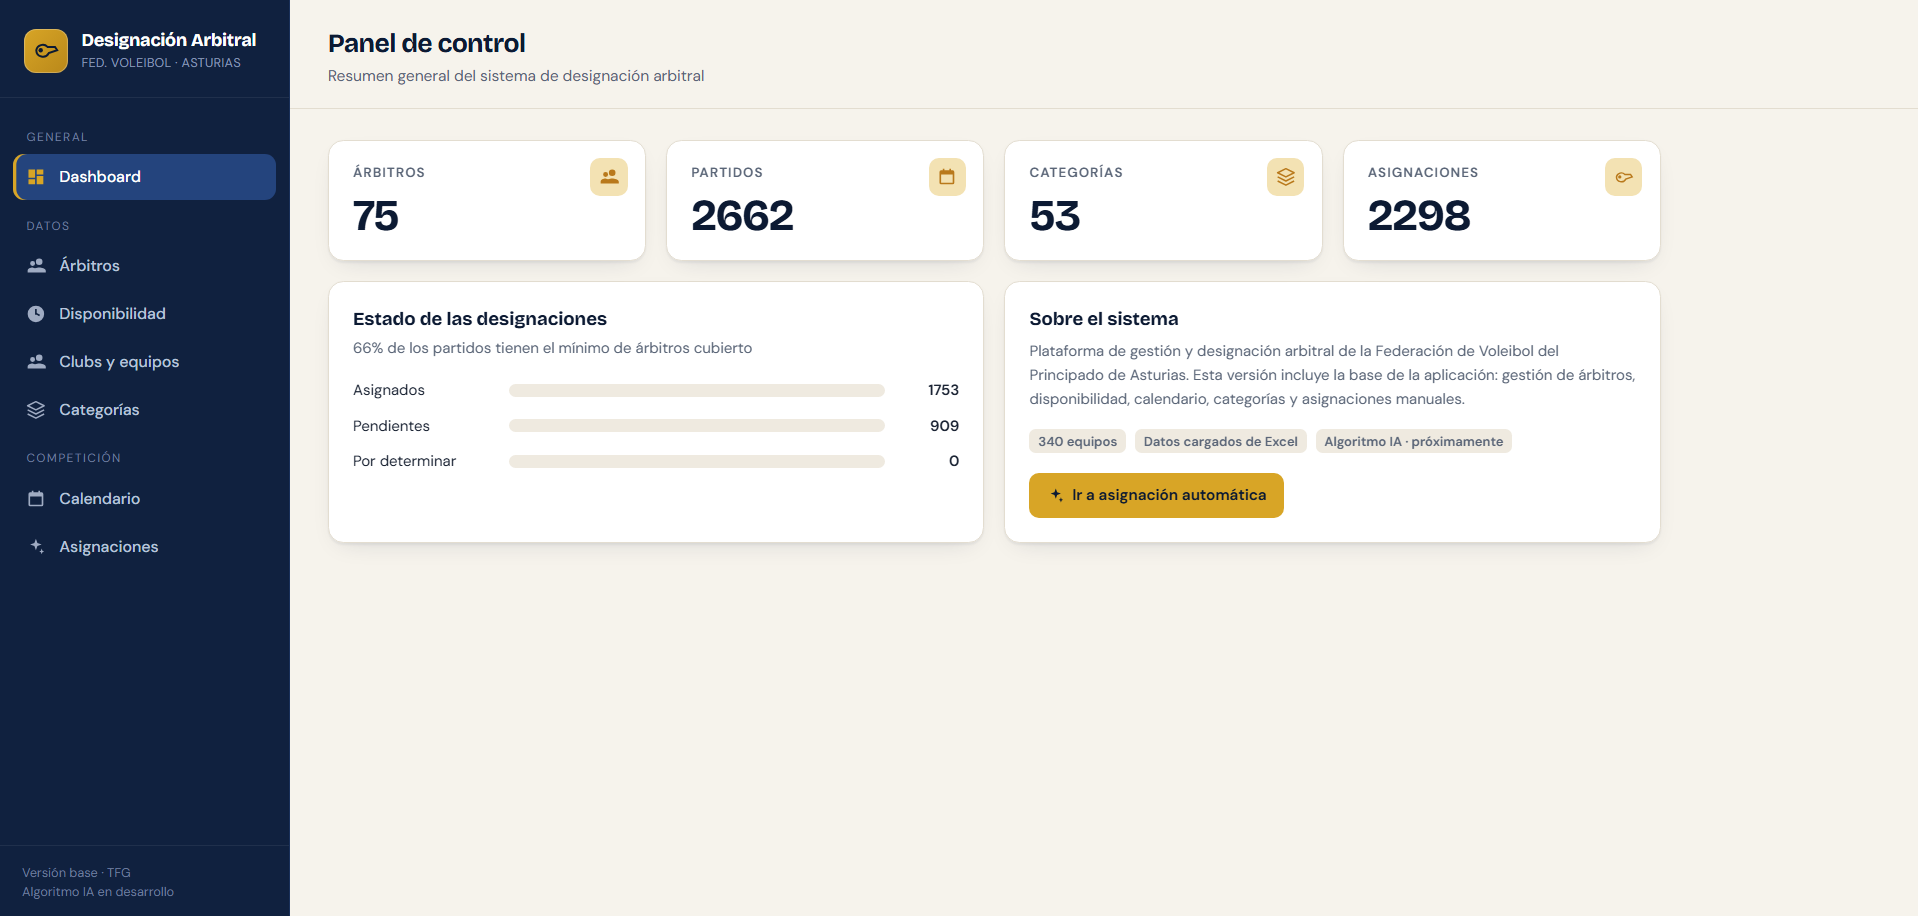
\includegraphics[width=\textwidth]{dashboard.png}
\caption{Panel de control de la aplicación, con los contadores generales y el estado de las designaciones.}
\label{fig:dashboard}
\fuente{elaboración propia (captura de la aplicación).}
\end{figure}

\subsection{Árbitros}

La sección de árbitros (Figura~\ref{fig:arbitros}) es donde se gestiona el cuerpo arbitral. Lo que más me gusta de esta pantalla es el mapa: como ya tengo geolocalizados a los árbitros y los polideportivos, los pinto todos sobre un mapa de Asturias, con un color para los árbitros y otro para las sedes. Eso ayuda muchísimo a entender por qué el sistema toma ciertas decisiones —se ve a simple vista qué árbitros están cerca de cada zona— y a detectar si alguna dirección se ha geocodificado mal. Debajo del mapa hay una tabla con cada árbitro, su código, su nivel, su localidad y su estado, con un buscador y un filtro por nivel.

\begin{figure}[ht]
\centering
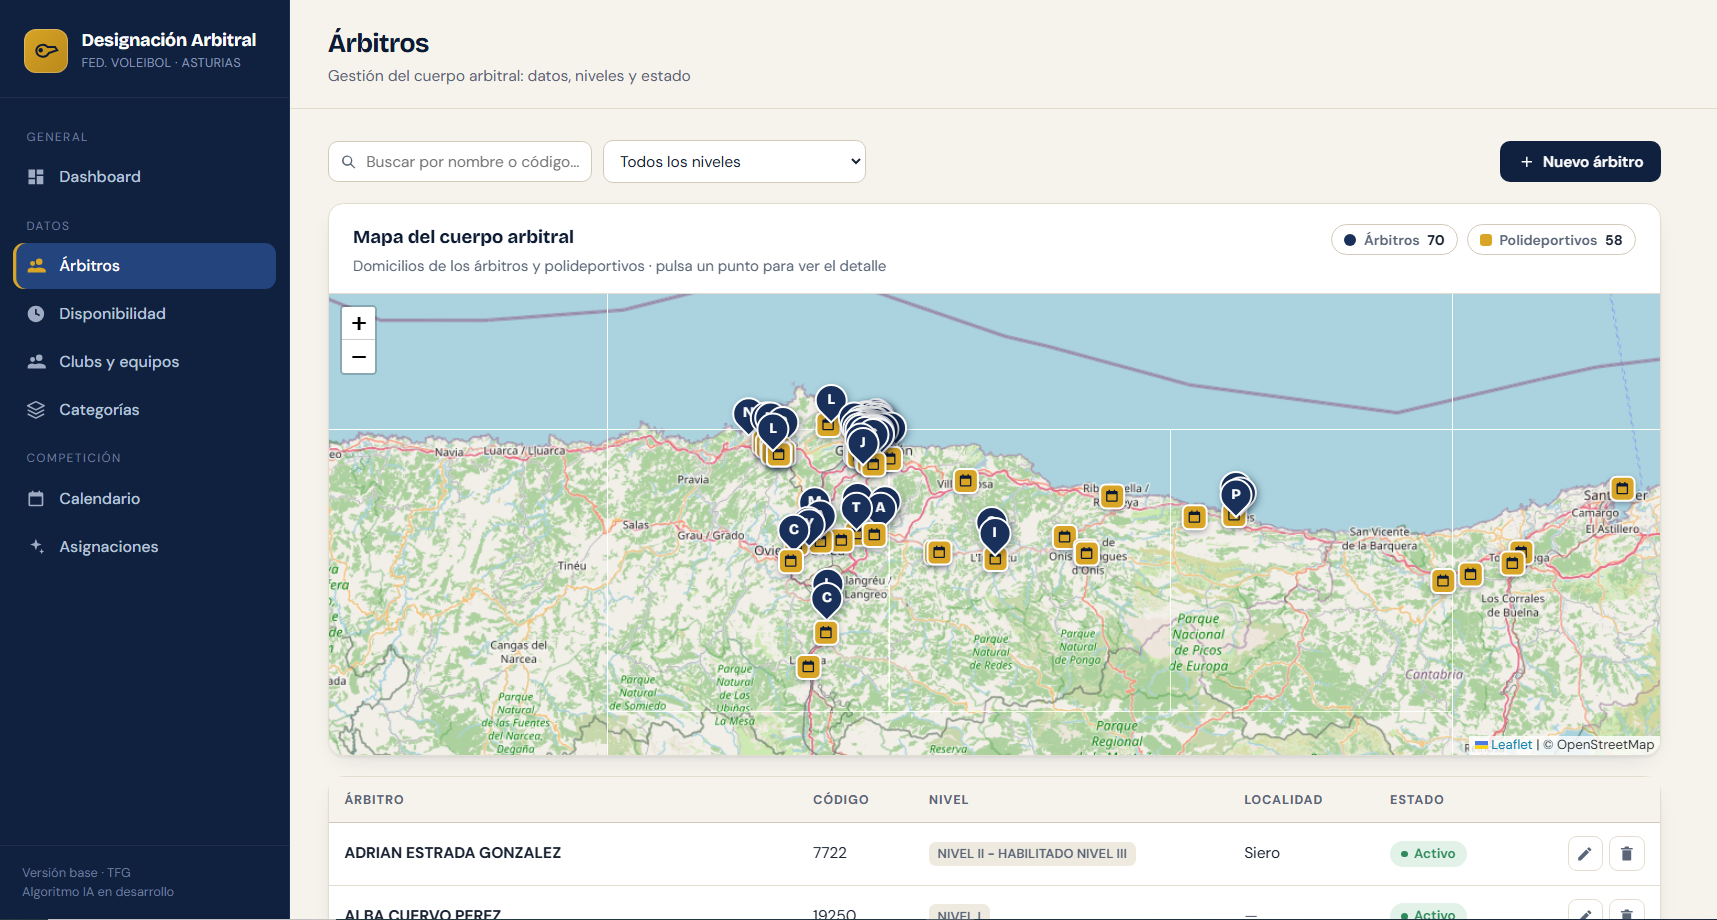
\includegraphics[width=\textwidth]{arbitros.png}
\caption{Gestión de árbitros, con el mapa del cuerpo arbitral (árbitros y polideportivos geolocalizados) y la tabla de detalle.}
\label{fig:arbitros}
\fuente{elaboración propia (captura de la aplicación).}
\end{figure}

\subsection{Disponibilidad}

Esta es seguramente la pantalla más importante de la parte de datos, porque la disponibilidad es la restricción que más manda en el algoritmo. Se elige un árbitro y aparece un calendario mensual (Figura~\ref{fig:disp1}). Cada día se puede marcar de golpe con uno de los tres estados —con transporte, sin transporte o no disponible— o, si se pincha en un día concreto, se abre un detalle (Figura~\ref{fig:disp2}) para afinar franja por franja: 09:00--12:00, 12:00--15:00, 15:00--18:00 y 18:00--22:00. Esas cuatro franjas son las que después usa el algoritmo para decidir si un árbitro puede o no pitar un partido a una hora dada.

La distinción entre «con transporte» y «sin transporte» es clave y no es un capricho de la interfaz: marca toda la lógica del coche compartido que explico más adelante. Un árbitro «con transporte» va en su coche y, además, puede llevar a compañeros; uno «sin transporte» solo puede ir a sedes que tenga cerca o que alguien con coche le recoja.

\begin{figure}[ht]
\centering
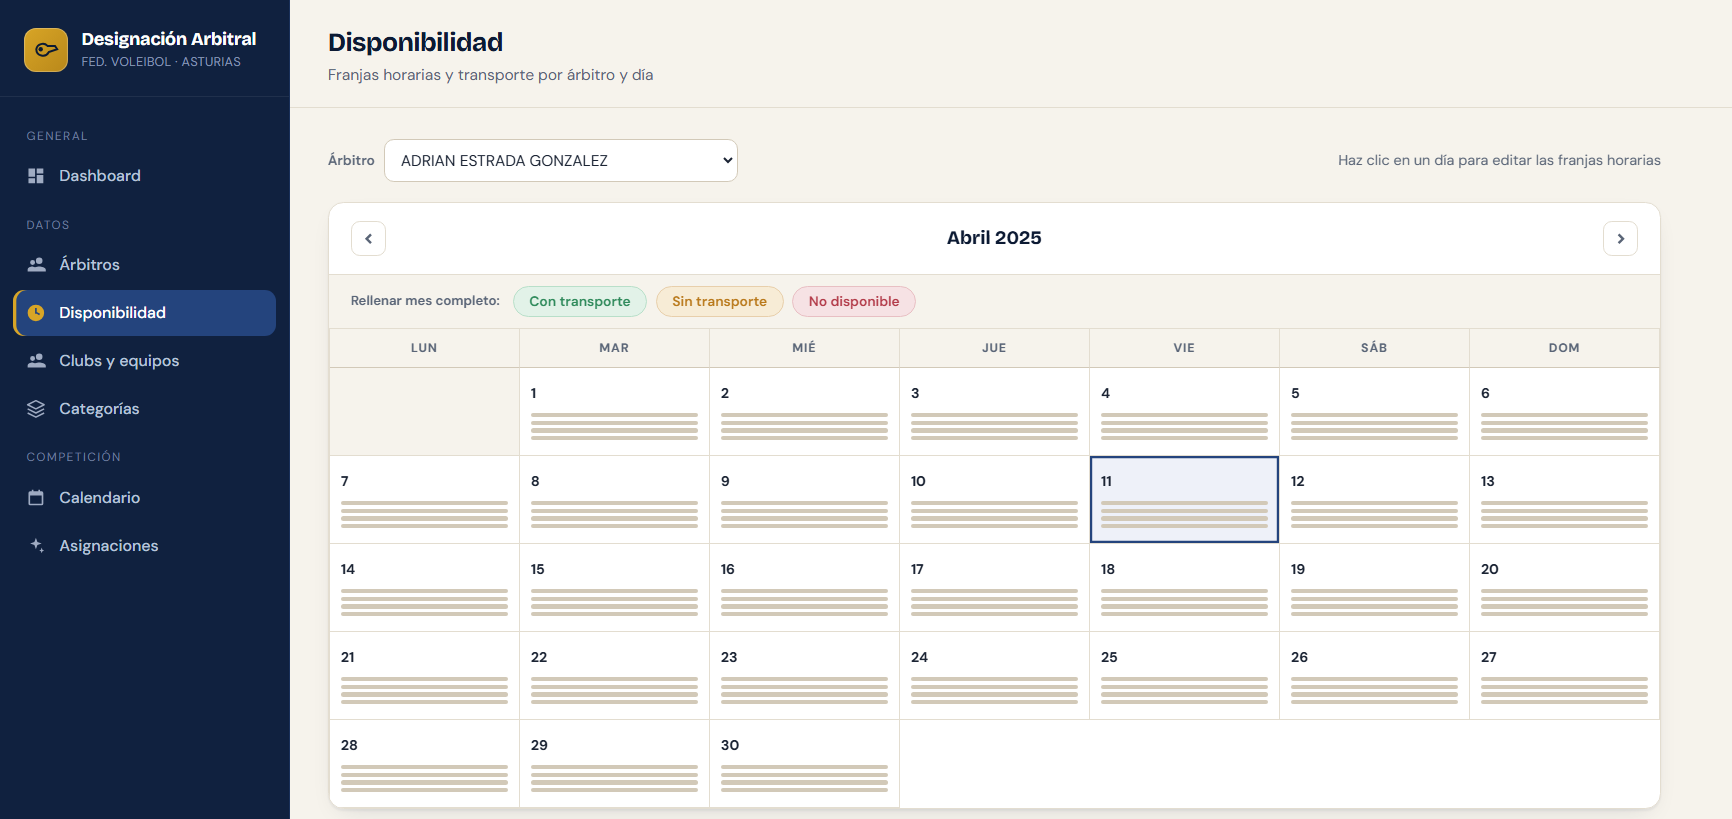
\includegraphics[width=\textwidth]{disponibilidad1.png}
\caption{Calendario mensual de disponibilidad de un árbitro, con los tres estados posibles por día.}
\label{fig:disp1}
\fuente{elaboración propia (captura de la aplicación).}
\end{figure}

\begin{figure}[ht]
\centering
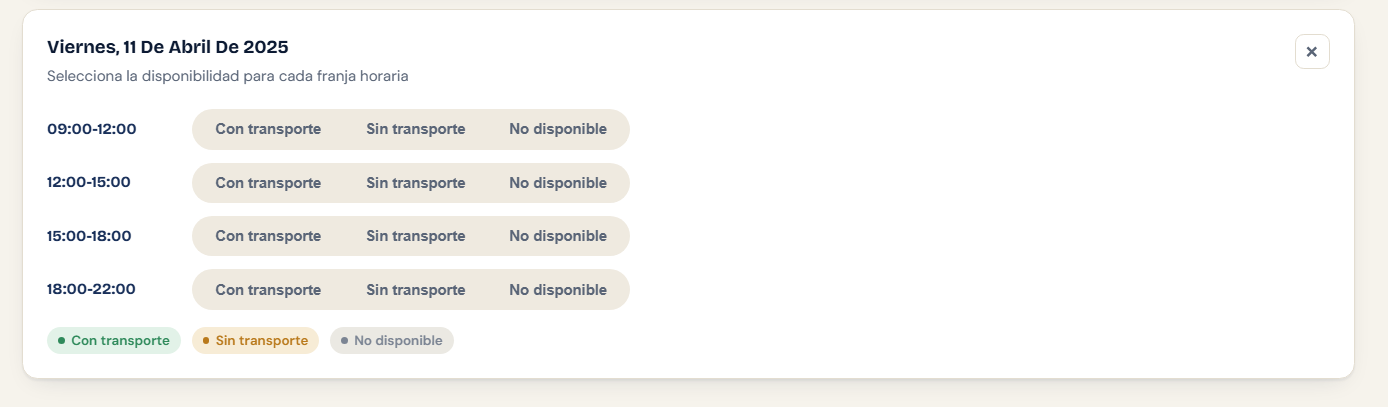
\includegraphics[width=0.85\textwidth]{disponibilidad2.png}
\caption{Detalle de un día: la disponibilidad se fija de forma independiente para cada una de las cuatro franjas horarias.}
\label{fig:disp2}
\fuente{elaboración propia (captura de la aplicación).}
\end{figure}

\subsection{Clubs, equipos y categorías}

Estas dos pantallas son más de catálogo, pero importan para el algoritmo. La de clubs y equipos (Figura~\ref{fig:clubs}) muestra cada club de la federación con sus equipos asociados; sirve, entre otras cosas, para tener identificado quién es quién de cara a los conflictos de interés. La de categorías (Figura~\ref{fig:categorias}) es más técnica: cada categoría define qué árbitros necesita (primero, segundo y anotador), el nivel mínimo de cada rol, el número mínimo de árbitros y —esto es importante— una \emph{prioridad}. Esa prioridad es la que le dice al algoritmo qué partidos son innegociables (los de máxima categoría, que tienen que salir sí o sí) y cuáles se pueden dejar a medias si no llegan los árbitros. Lo retomo cuando hable del objetivo del modelo.

\begin{figure}[ht]
\centering

\includegraphics[width=\textwidth]{clubs.png}
\caption{Catálogo de clubs de la federación con sus equipos asociados.}
\label{fig:clubs}
\fuente{elaboración propia (captura de la aplicación).}
\end{figure}

\begin{figure}[ht]
\centering
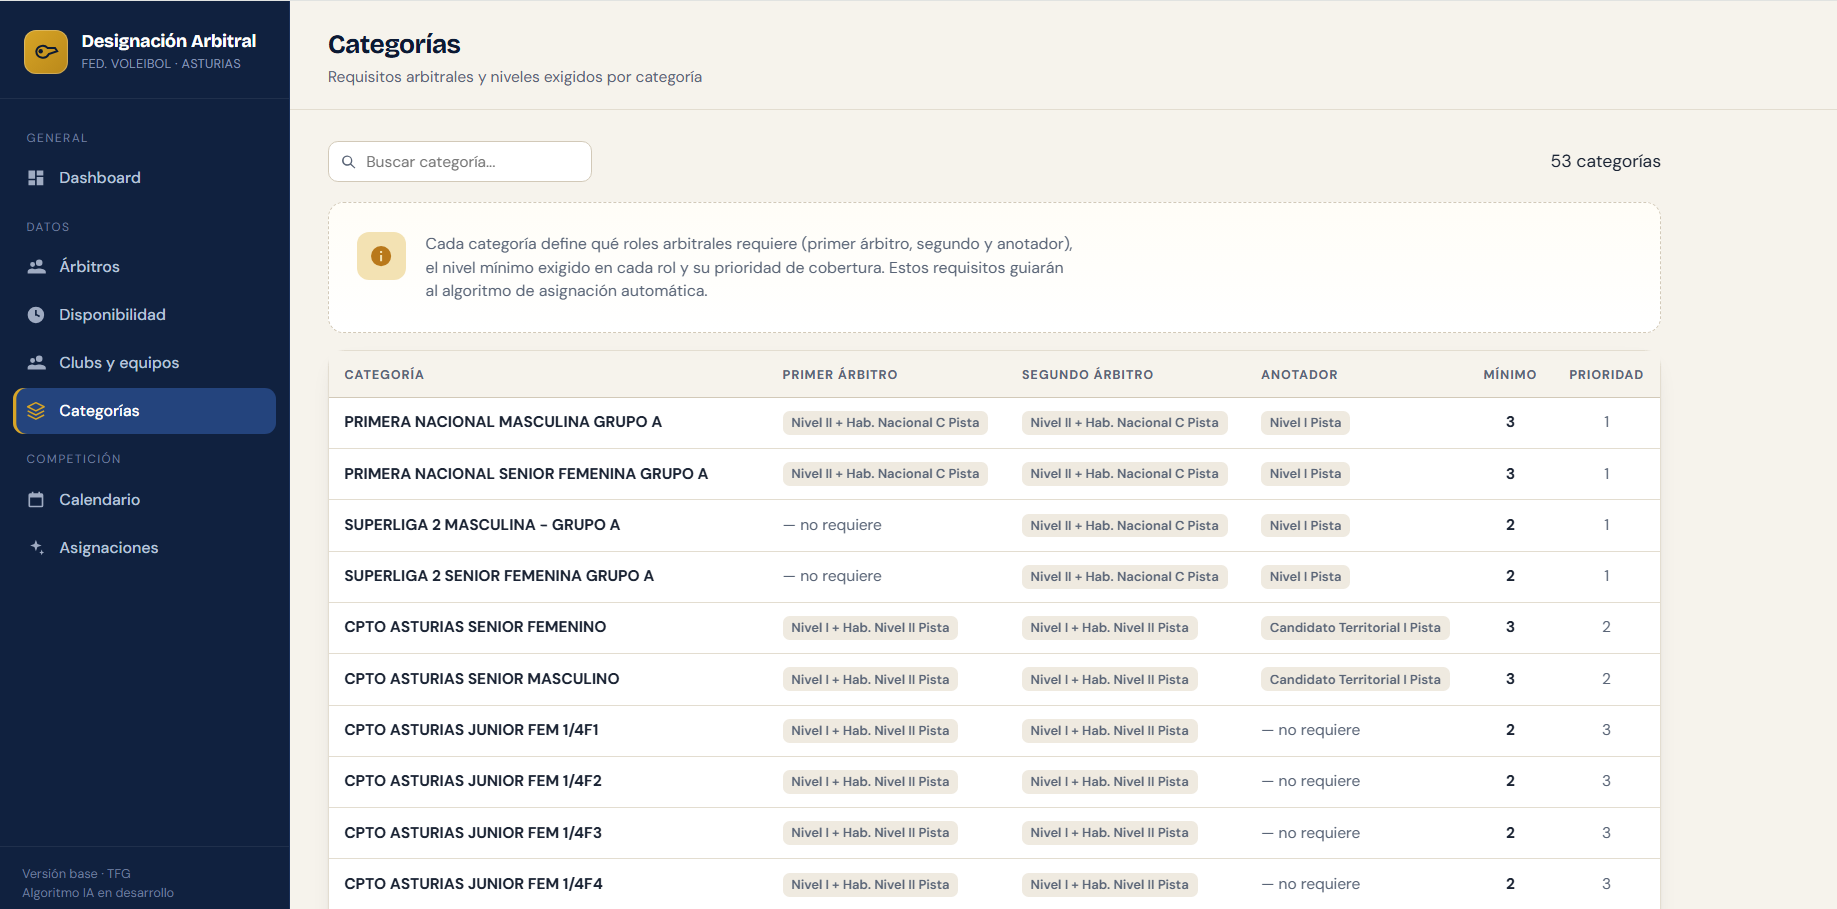
\includegraphics[width=\textwidth]{categorias.png}
\caption{Categorías de competición: roles exigidos, nivel mínimo por rol, número mínimo de árbitros y prioridad.}
\label{fig:categorias}
\fuente{elaboración propia (captura de la aplicación).}
\end{figure}

\subsection{Calendario}

El calendario (Figura~\ref{fig:calendario}) es la lista de partidos programados con su estado de designación. Se puede filtrar por fechas, por categoría y por estado (pendiente, asignado, por determinar), y desde aquí también se puede entrar a designar un partido a mano. Es la vista que conecta con la realidad: estos son los partidos que de verdad hay que cubrir.

\begin{figure}[ht]
\centering
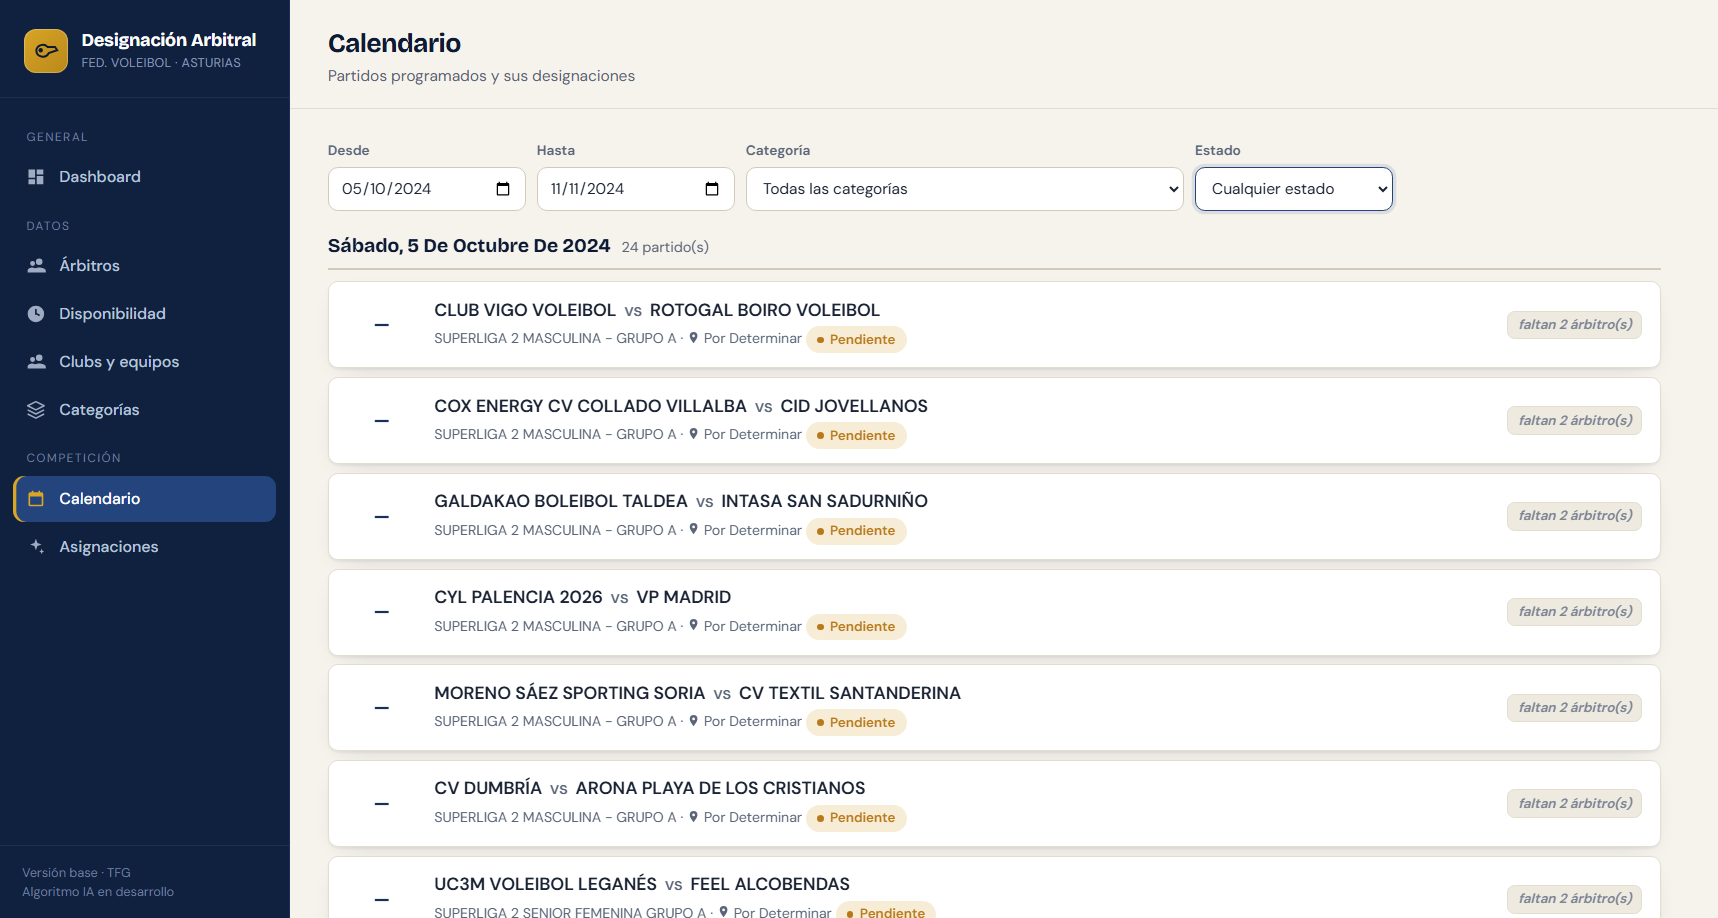
\includegraphics[width=\textwidth]{calendario.png}
\caption{Calendario de partidos programados, con filtros por fecha, categoría y estado de designación.}
\label{fig:calendario}
\fuente{elaboración propia (captura de la aplicación).}
\end{figure}

\subsection{Asignaciones: la designación automática}

Y llegamos a la pantalla estrella, la de asignaciones (Figura~\ref{fig:desig1}), que es donde se lanza la designación automática. El funcionamiento es directo: se elige un rango de fechas («Desde» / «Hasta»), se pulsa «Generar designación» y el motor se pone a trabajar. Solo entran en el cálculo los partidos que tienen todos los datos necesarios (categoría, hora y sede); el resto se queda fuera porque no se pueden designar. El resultado es una propuesta que se previsualiza —no se guarda todavía— y que el usuario revisa antes de pulsar «Publicar» para que se vuelque al calendario. También se pueden borrar las designaciones de ese rango de un tirón.

\begin{figure}[ht]
\centering
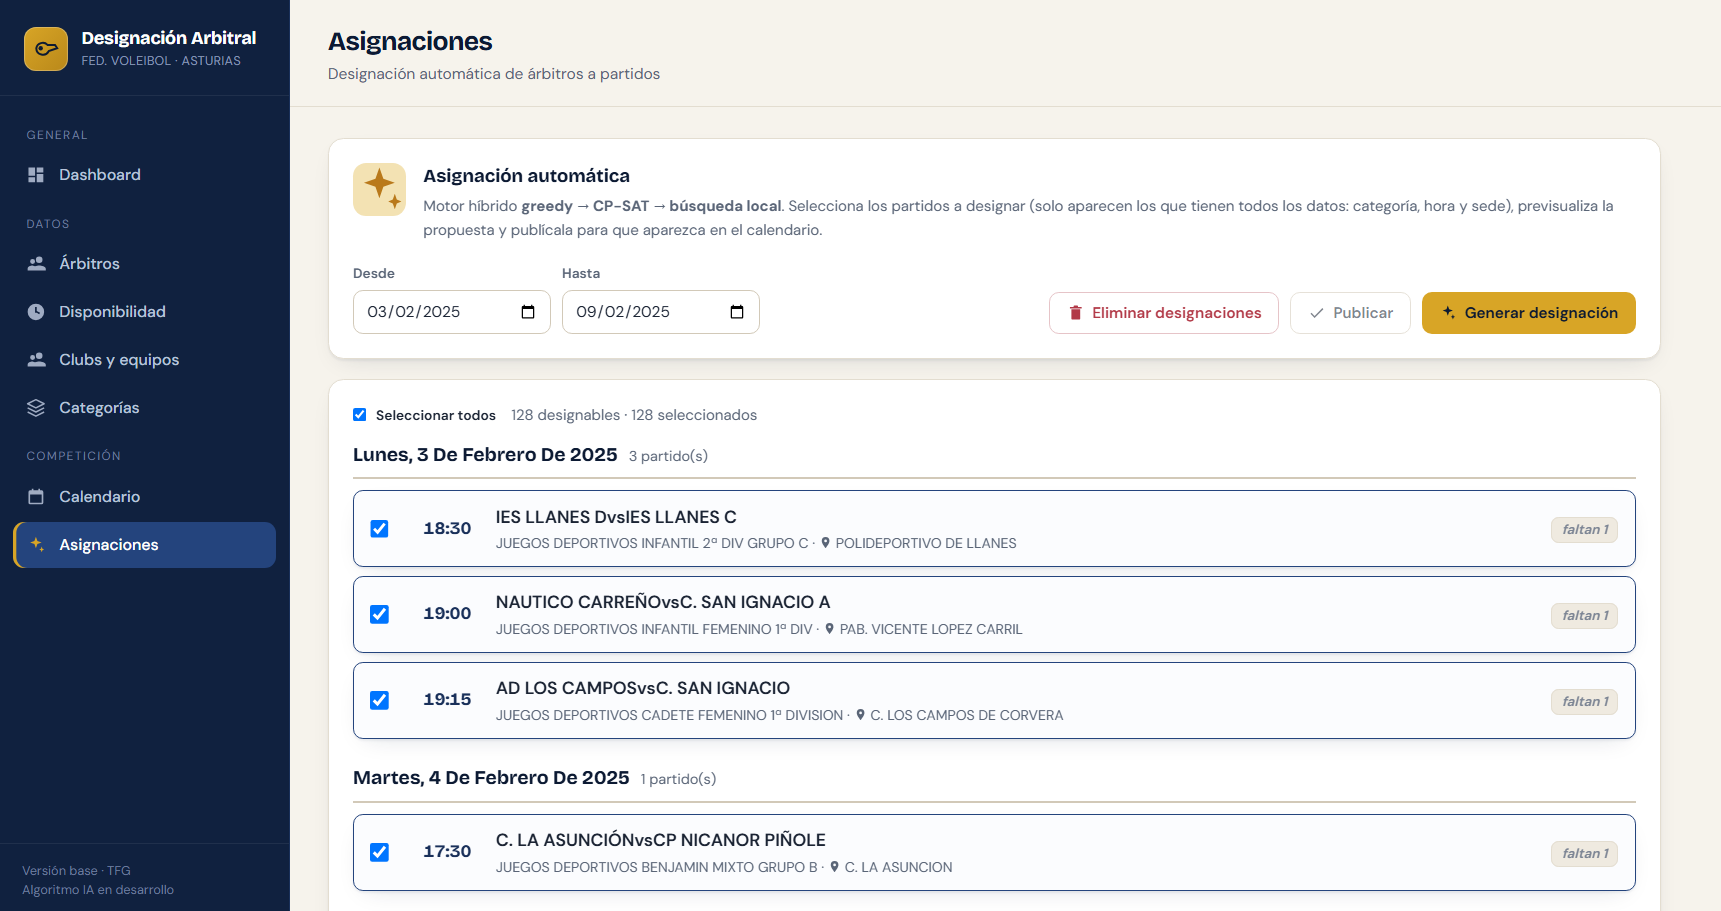
\includegraphics[width=\textwidth]{designaciones1.png}
\caption{Pantalla de designación automática: selección del rango de fechas y lista de partidos designables.}
\label{fig:desig1}
\fuente{elaboración propia (captura de la aplicación).}
\end{figure}

Lo interesante viene tras generar la designación. Como se ve en la Figura~\ref{fig:desig2}, la aplicación enseña tres tarjetas de métricas —cobertura, kilómetros totales y árbitros usados— y, debajo, un «Detalle de la optimización» que es básicamente una radiografía de lo que ha hecho el motor por dentro: qué fases se han ejecutado (greedy, CP-SAT, búsqueda local), cuánto ha tardado cada una, cuántas variables ha manejado el solver y si ha encontrado el óptimo. Quise que esto se viera porque una de las gracias del sistema es que no es una caja negra: el responsable de designaciones puede ver que, por ejemplo, sobre 128 partidos se han cubierto el 90,2\,\% de los roles, recorriendo 1179,1 km, usando 45 árbitros con una carga de entre 1 y 7 partidos. Sobre estos números vuelvo en la Sección~\ref{sec:resultados}.

\begin{figure}[ht]
\centering
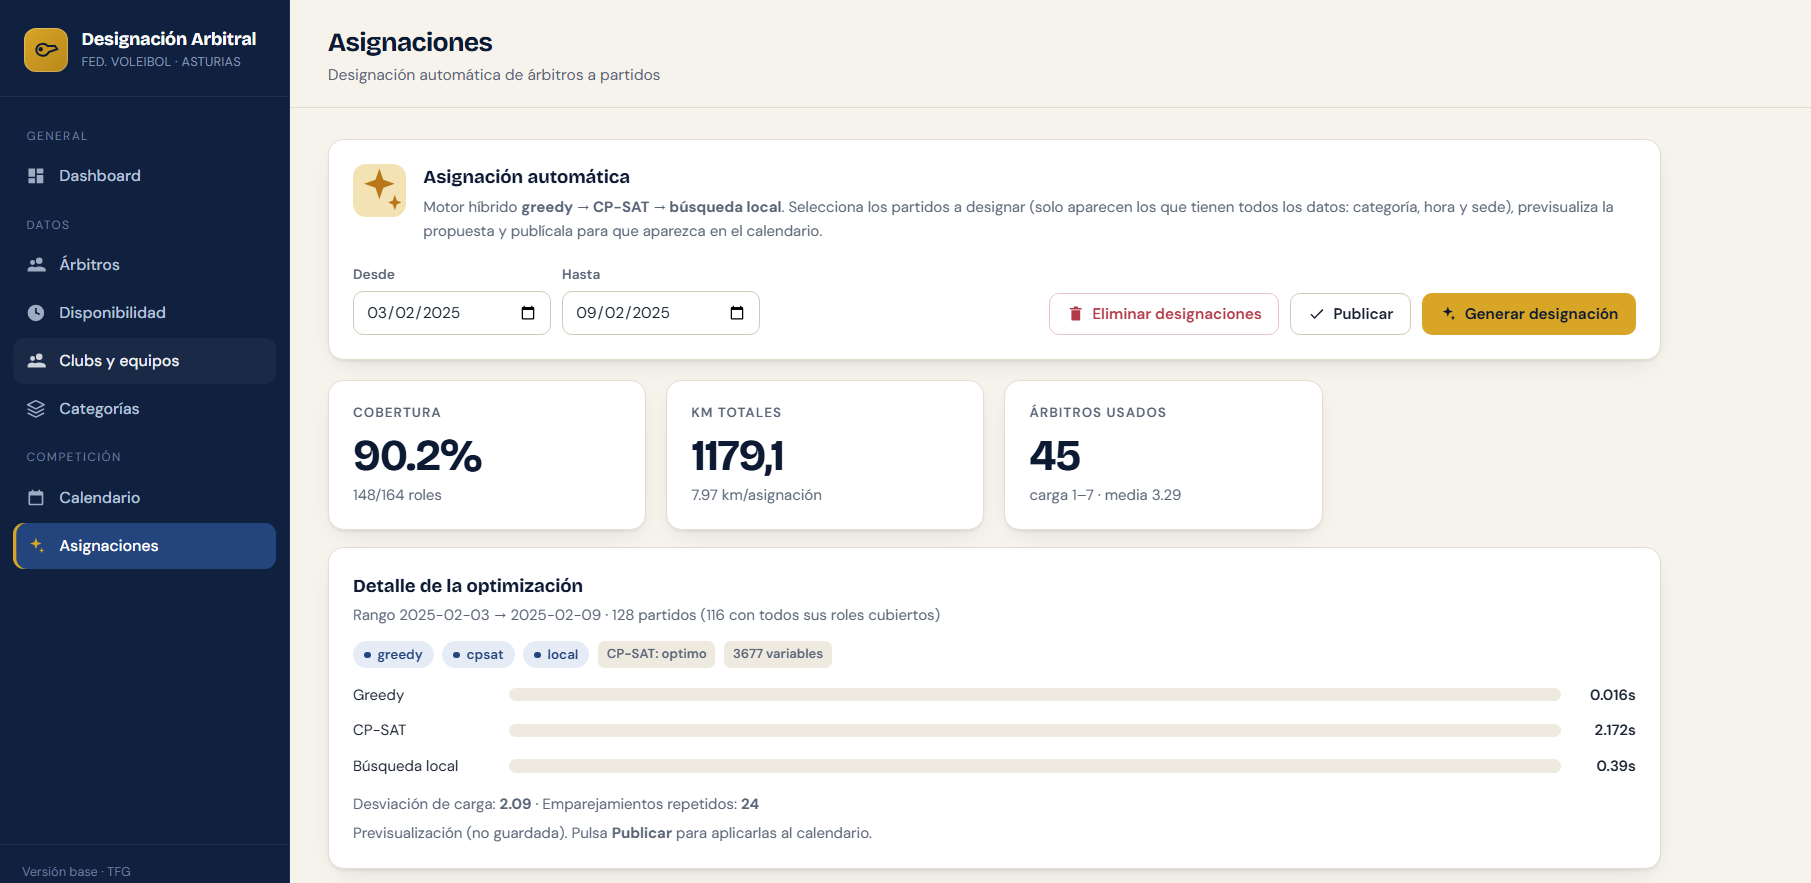
\includegraphics[width=\textwidth]{designaciones2.png}
\caption{Resultado de la designación automática: métricas de cobertura, kilometraje y equidad, y detalle de las fases del algoritmo con sus tiempos.}
\label{fig:desig2}
\fuente{elaboración propia (captura de la aplicación).}
\end{figure}

Por último, bajo las métricas aparece la lista de partidos con sus árbitros ya asignados (Figura~\ref{fig:desig3}). Cada árbitro se muestra con una etiqueta de color y, si procede, con información de cómo se desplaza: si va en su coche, si le lleva un compañero (y quién) o si va andando. Toda esa información de transporte sale del análisis de itinerarios que explico en la Sección~\ref{sec:coche}.

\begin{figure}[ht]
\centering
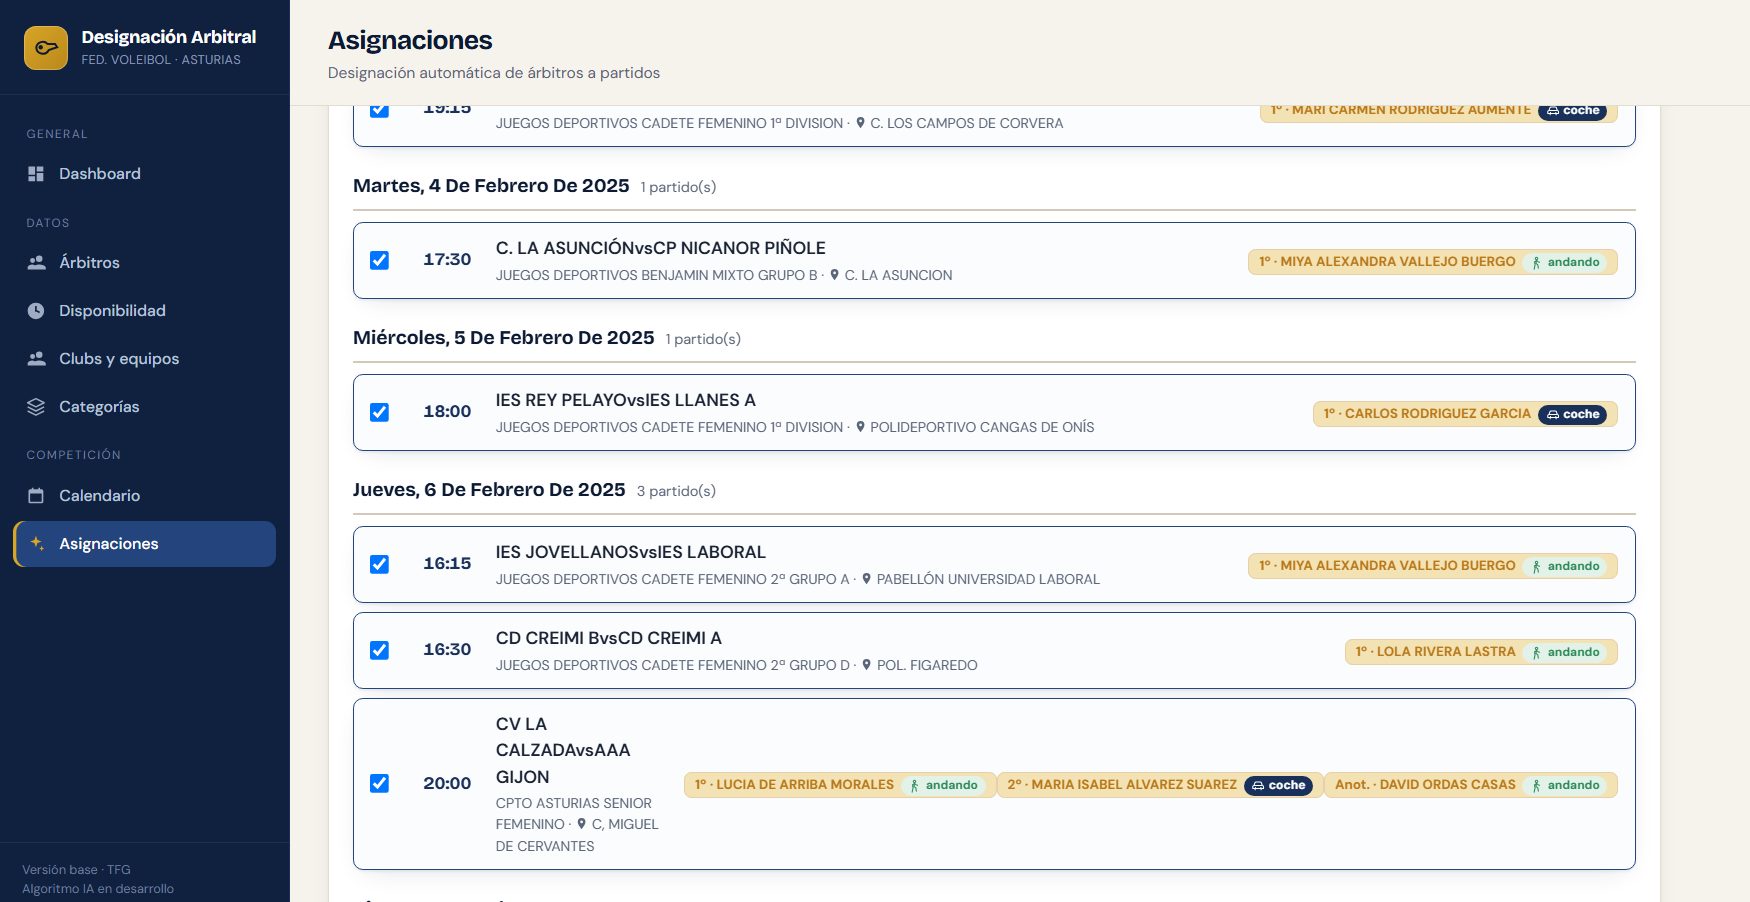
\includegraphics[width=\textwidth]{designaciones3.png}
\caption{Detalle de la asignación por partido: cada árbitro aparece con su rol y con la forma en que se desplaza a la sede.}
\label{fig:desig3}
\fuente{elaboración propia (captura de la aplicación).}
\end{figure}

\section{Modelado formal del problema}
\label{sec:modelo}

Una vez vista la aplicación por fuera, toca formalizar qué es exactamente lo que el algoritmo tiene que resolver. Aunque al final use un enfoque híbrido, me vino muy bien escribir el problema como un modelo de optimización, porque obliga a dejar claro qué son las variables, qué restricciones hay y qué se quiere minimizar.

\subsection{Conjuntos y variables}

Tengo un conjunto de árbitros y un conjunto de partidos en un rango de fechas. Cada partido $p$ exige una serie de \emph{roles} (primero, segundo y/o anotador, según su categoría), y cada rol $r$ pide un nivel mínimo. La variable de decisión principal es binaria:
\begin{equation}
x_{p,r,a} =
\begin{cases}
1 & \text{si el árbitro } a \text{ cubre el rol } r \text{ del partido } p,\\
0 & \text{en caso contrario.}
\end{cases}
\end{equation}

No genero esta variable para todas las combinaciones posibles, sino solo para los \emph{candidatos válidos}: árbitros que ese día y a esa hora están disponibles, que alcanzan el nivel del rol y que pueden llegar a la sede. Eso reduce muchísimo el tamaño del problema, y lo explico en detalle en la Sección~\ref{sec:instancia}. Además, para cada rol defino una variable de holgura $u_{p,r}\in\{0,1\}$ que vale 1 si ese rol se queda \emph{sin cubrir}. Esto es importante: en la realidad puede que no haya árbitros para todo, así que en vez de hacer el problema infactible, permito dejar roles sin cubrir pero penalizándolo en el objetivo.

\subsection{Restricciones}

Las restricciones duras del modelo son las siguientes:

\paragraph{Cobertura de cada rol.} Cada rol requerido lo cubre exactamente un árbitro, o bien se queda sin cubrir:
\begin{equation}
\sum_{a \in C_{p,r}} x_{p,r,a} + u_{p,r} = 1 \qquad \forall (p,r),
\label{eq:cobertura}
\end{equation}
donde $C_{p,r}$ es el conjunto de candidatos válidos para ese rol.

\paragraph{Un árbitro, un rol por partido.} Un mismo árbitro no puede ocupar dos roles del mismo partido:
\begin{equation}
\sum_{r} x_{p,r,a} \le 1 \qquad \forall (p,a).
\end{equation}

\paragraph{Sin solapes horarios.} Si dos partidos $p_1$ y $p_2$ se pisan en el tiempo para un mismo árbitro —teniendo en cuenta no solo la duración sino también lo que tarda en viajar de una sede a otra—, no se le pueden asignar los dos:
\begin{equation}
\sum_{r} x_{p_1,r,a} + \sum_{r} x_{p_2,r,a} \le 1 \qquad \forall a, \ \forall (p_1,p_2) \text{ en conflicto}.
\end{equation}

\paragraph{Coche compartido.} Un árbitro «sin transporte» que vive lejos de la sede solo puede ir si en ese mismo partido hay asignado un árbitro «con transporte» que viva cerca de él y pueda recogerlo. Si llamo $L_{p}$ al conjunto de candidatos «lejos» del partido y $D_{p,a}$ a los conductores que podrían recoger al árbitro $a$:
\begin{equation}
\sum_{r} x_{p,r,a} \le \sum_{c \in D_{p,a}} \sum_{r'} x_{p,r',c} \qquad \forall p, \ \forall a \in L_{p}.
\end{equation}

\subsection{Función objetivo}

El objetivo junta tres cosas que quiero a la vez: gastar pocos kilómetros, cubrir el máximo de partidos (sobre todo los importantes) y repartir la carga con equidad. Lo escribo como una única función a minimizar:
\begin{equation}
\min \ \underbrace{\sum_{p,r,a} d_{p,a}\, x_{p,r,a}}_{\text{kilómetros}} \;+\; \underbrace{\sum_{p,r} w_{p}\, u_{p,r}}_{\text{penalización por no cubrir}} \;+\; \underbrace{W_{eq}\cdot \text{carga}_{\max}}_{\text{equidad}},
\label{eq:objetivo}
\end{equation}
donde $d_{p,a}$ es la distancia del árbitro $a$ a la sede del partido $p$, $w_p$ es una penalización que depende de la prioridad de la categoría, y $\text{carga}_{\max}$ es el número de partidos del árbitro más cargado.

La clave está en los pesos $w_p$. No todos los partidos valen lo mismo: dejar sin árbitro un partido de máxima categoría es gravísimo, mientras que dejar a medias uno de la categoría más baja un fin de semana saturado es asumible. Por eso uso una penalización \emph{escalonada} por prioridad, con órdenes de magnitud muy separados para que la jerarquía se respete siempre por encima de los kilómetros. Concretamente, los pesos que uso son los de la Tabla~\ref{tab:pesos}.

\begin{table}[ht]
\centering
\caption{Pesos de la función objetivo. Los órdenes de magnitud están separados a propósito para que cubrir los partidos importantes mande siempre por encima de ahorrar kilómetros.}
\label{tab:pesos}
\begin{tabular}{@{}p{7.5cm}r@{}}
\toprule
{\bf Concepto} & {\bf Peso} \\
\midrule
Rol sin cubrir de una categoría de prioridad 1 & 1\,000\,000 \\
Partido de prioridad 2--9 que se queda sin ningún árbitro & 100\,000 \\
Cualquier otro rol sin cubrir & 2\,000 \\
Equidad (carga máxima) & 5 \\
Cada kilómetro recorrido & 1 \\
\bottomrule
\end{tabular}
\fuente{elaboración propia.}
\end{table}

Con estos pesos, el solver primero se asegura de cubrir todo lo de prioridad 1, luego de que ningún partido de prioridad media se quede vacío del todo, después de cubrir el resto de roles, y solo entonces, dentro de lo que le quede de margen, se pone a recortar kilómetros y a equilibrar la carga. Es una forma sencilla pero efectiva de meter una jerarquía de objetivos en una sola función lineal.

\section{Preparación de la instancia}
\label{sec:instancia}

Antes de que cualquiera de las tres fases toque nada, hay un paso previo que hace gran parte del trabajo sucio: construir la \emph{instancia} del problema a partir de la base de datos. Esto vive en \texttt{datos.py} y es la entrada común de las tres fases. Aquí es donde se decide quién es candidato a qué, que es justo lo que hace que el problema sea manejable.

\subsection{El modelo temporal}

Para saber si dos partidos se solapan para un árbitro no basta con mirar la hora de inicio. Un partido «ocupa» al árbitro un rato antes (tiene que llegar con antelación) y un rato durante (lo que dura). Modelé esto así: la antelación es de una hora en los partidos de prioridad 1 y de media hora en el resto; la duración media es de hora y media en las categorías altas y de una hora en las bajas. Con eso, cada partido tiene una ventana de ocupación. Dos partidos del mismo día solapan para un árbitro si esas ventanas se cruzan o si, aun sin cruzarse, no le da tiempo a viajar de una sede a otra. Y aquí es donde el medio de transporte importa: el tiempo de viaje se calcula a la velocidad del coche (70 km/h) si el árbitro tiene transporte, o a velocidad de andar (5 km/h) si no. La función que decide el solape es la siguiente:

\begin{lstlisting}[caption={Detección de solape entre dos partidos para un mismo árbitro, teniendo en cuenta el tiempo de viaje (\texttt{datos.py}).},label={lst:conflictan}]
def conflictan(p1, p2, velocidad_kmh=VELOCIDAD_KMH):
    """True si un mismo árbitro no puede hacer ambos partidos (solape o viaje)."""
    if p1.ini_ocup is None or p2.ini_ocup is None:
        return False
    primero, segundo = (p1, p2) if p1.inicio_min <= p2.inicio_min else (p2, p1)
    # El segundo debe empezar (con su antelación) tras terminar el primero + viaje.
    return segundo.ini_ocup < primero.fin_ocup + viaje_min(
        primero.sede, segundo.sede, velocidad_kmh
    )
\end{lstlisting}

\subsection{El cálculo de candidatos}

Lo más importante de esta fase es decidir, para cada partido y cada rol, qué árbitros son candidatos válidos. Un árbitro entra como candidato si cumple tres cosas: está disponible ese día y franja (con o sin transporte), alcanza el nivel mínimo del rol, y no tiene un conflicto de interés con ninguno de los dos equipos. Pero además, a cada candidato le pongo una \emph{etiqueta} según cómo puede llegar a la sede, y esto es el germen del coche compartido:

\begin{itemize}
\item {\bf «con»}: tiene transporte, va en su coche y además puede llevar a otros.
\item {\bf «cerca»}: no tiene transporte, pero la sede le pilla cerca (a menos de 10 km), así que puede ir por sus medios (andando).
\item {\bf «lejos»}: no tiene transporte y la sede le pilla lejos. Este solo vale si en el partido hay un conductor que viva cerca de él y pueda recogerlo; si no, no puede llegar y lo descarto.
\end{itemize}

El fragmento que calcula los candidatos y sus etiquetas es este:

\begin{lstlisting}[caption={Cálculo de candidatos por (partido, rol) y su etiqueta de transporte (\texttt{datos.py}).},label={lst:candidatos}]
for rol, rango_min in p.roles:
    lista, tipo = [], {}
    for a in arbitros:
        estado = a.disp.get((p.fecha, p.franja))
        if estado not in ("con_transporte", "sin_transporte"):
            continue                                   # no disponible
        if not niveles.cumple_nivel(a.rango, rango_min):
            continue                                   # no alcanza el nivel
        if conflictos.hay_conflicto(a.id, p.local, p.visitante):
            continue                                   # conflicto de interés
        dist = _distancia(a, p.sede)
        if estado == "con_transporte":
            t = "con"
        else:
            if dist is None:
                continue            # sin coords no se puede compartir coche
            t = "cerca" if dist <= umbral else "lejos"
        lista.append((a.idx, dist))
        tipo[a.idx] = t
\end{lstlisting}

Después de esto, hay un repaso final que descarta los candidatos «lejos» que no tengan en su partido ningún conductor cercano posible: si nadie puede recogerlos, no tiene sentido ni considerarlos. Esa poda deja la instancia limpia y lista para las tres fases.

\section{El algoritmo de asignación en tres fases}
\label{sec:algoritmo}

Aquí está el corazón del trabajo. Como expliqué en el estado del arte, decidí un enfoque híbrido en la línea de las matheurísticas: una heurística golosa que construye una primera solución, el solver exacto CP-SAT que la optimiza, y una búsqueda local que la pule. Las tres fases se encadenan en \texttt{pipeline.py}, y entre fase y fase me quedo siempre con la mejor solución según un criterio de calidad: primero cobertura (cuantos más roles cubiertos, mejor) y, a igualdad de cobertura, menos kilómetros. La Figura~\ref{fig:fases} resume el flujo.

\begin{figure}[ht]
\centering
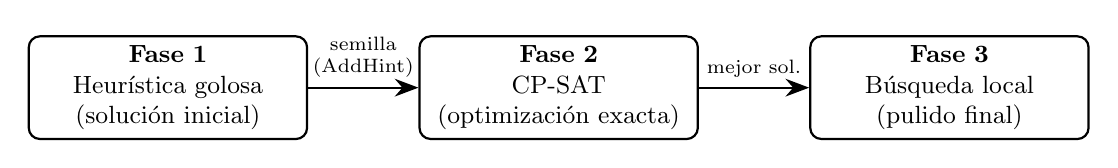
\begin{tikzpicture}[
  node distance=10mm,
  fase/.style={rectangle, rounded corners, draw, thick, align=center, minimum height=13mm, text width=33mm, font=\small},
  flecha/.style={-{Stealth[length=3mm]}, thick}
]
\node[fase] (g) {{\bf Fase 1}\\Heurística golosa\\(solución inicial)};
\node[fase, right=14mm of g] (c) {{\bf Fase 2}\\CP-SAT\\(optimización exacta)};
\node[fase, right=14mm of c] (l) {{\bf Fase 3}\\Búsqueda local\\(pulido final)};
\draw[flecha] (g) -- node[above, font=\scriptsize, align=center]{semilla\\(AddHint)} (c);
\draw[flecha] (c) -- node[above, font=\scriptsize]{mejor sol.} (l);
\end{tikzpicture}
\caption{Las tres fases del motor de asignación. La solución golosa siembra al solver CP-SAT, y la búsqueda local pule el mejor resultado obtenido.}
\label{fig:fases}
\fuente{elaboración propia.}
\end{figure}

\subsection{Fase 1: heurística golosa}

La primera fase (en \texttt{greedy.py}) construye una solución desde cero tomando decisiones golosas. La gracia no está tanto en cada decisión individual como en el \emph{orden} en que ataco los partidos, que es lo que hace que, si faltan árbitros, los que se queden sin cubrir sean los menos importantes. El orden tiene tres pasos:

\begin{enumerate}
\item Primero cubro por completo los partidos de prioridad 1 (todos sus roles): estos son innegociables.
\item Después garantizo \emph{al menos un} árbitro en cada partido restante, recorriéndolos por orden de prioridad. Así, si me quedo corto de árbitros, los huecos caen en las categorías bajas.
\item Por último, vuelvo sobre el resto para completar los roles que falten.
\end{enumerate}

\begin{lstlisting}[caption={Orden de asignación de la fase golosa según la prioridad de la categoría (\texttt{greedy.py}).},label={lst:greedy-orden}]
# 1) Prioridad 1: cobertura completa (todos los roles, obligatorios).
for p in prio1:
    completar(p)
# 2) Resto: al menos un árbitro por partido, en orden de prioridad.
for p in resto:
    garantizar_uno(p)
# 3) Resto: completar los roles que falten.
for p in resto:
    completar(p)
\end{lstlisting}

Dentro de cada partido, a la hora de elegir qué árbitro pongo en un rol, combino dos criterios: la distancia a la sede (quiero al más cercano) y la carga que lleva acumulada (quiero repartir). El que elijo es el que minimiza una clave que mezcla las dos cosas. Además, dentro de cada partido asigno primero los árbitros que van por sus medios (con coche o cercanos) y dejo para un segundo pase los «lejos», que solo acepto si ya hay en el partido un conductor que pueda recogerlos.

\begin{lstlisting}[caption={Elección del mejor candidato para un rol: distancia más un término de equidad (\texttt{greedy.py}).},label={lst:greedy-elegir}]
def _elegir(inst, p, rol, asignados_p, conductores_p, asig_arb, carga, permitir_lejos):
    mejor, mejor_clave = None, None
    for a_idx, dist in p.candidatos.get(rol, []):
        if a_idx in asignados_p:
            continue
        tipo = p.cand_tipo[rol].get(a_idx)
        if tipo == "lejos":
            if not permitir_lejos or not _hay_conductor_cercano(inst, conductores_p, a_idx):
                continue
        if _en_conflicto(inst, asig_arb, a_idx, p):     # solape horario
            continue
        d = dist if dist is not None else 9999.0
        clave = (d + 0.5 * carga[a_idx], carga[a_idx], d)   # distancia + equidad
        if mejor_clave is None or clave < mejor_clave:
            mejor_clave, mejor = clave, a_idx
    return mejor
\end{lstlisting}

Esta fase es rapidísima (centésimas de segundo) y deja una solución razonable, pero casi nunca óptima: por eso la uso como punto de partida de la fase siguiente, no como resultado final.

\subsection{Fase 2: optimización con CP-SAT}

Esta es la fase principal y la más potente. Uso CP-SAT, el solver de programación con restricciones de Google OR-Tools \cite{cpsat}, que mezcla un motor SAT con técnicas de programación entera y me deja escribir a la vez restricciones lógicas complicadas (como el coche compartido) y un objetivo numérico (los kilómetros). El modelo que construyo es el que formalicé en la Sección~\ref{sec:modelo}; aquí enseño cómo se traduce a código.

La restricción de cobertura de la ecuación~\eqref{eq:cobertura} es casi literal: para cada rol, la suma de las variables de sus candidatos más la holgura de «no cubierto» tiene que ser 1.

\begin{lstlisting}[caption={Variables y restricción de cobertura por rol (\texttt{cpsat.py}).},label={lst:cpsat-cobertura}]
for rol, _rango in p.roles:
    vars_rol = []
    for a_idx, dist in p.candidatos.get(rol, []):
        v = modelo.NewBoolVar(f"x_{p.idx}_{rol}_{a_idx}")
        x[(p.idx, rol, a_idx)] = v
        vars_rol.append(v)
        terminos.append((v, int(round(dist)) if dist is not None else COSTE_DESCONOCIDO))
        # ... (se registran también las estructuras de carga, tipo, etc.)
    u = modelo.NewBoolVar(f"u_{p.idx}_{rol}")     # holgura: rol sin cubrir
    no_cubierto[(p.idx, rol)] = u
    modelo.Add(sum(vars_rol) + u == 1)
\end{lstlisting}

La restricción de no solapamiento la genero recorriendo, para cada árbitro, todos los pares de partidos del mismo día que podría hacer, y comprobando con la función \texttt{conflictan} del Listado~\ref{lst:conflictan} (a la velocidad de su medio de transporte) si chocan:

\begin{lstlisting}[caption={Restricción de no solapamiento horario por árbitro (\texttt{cpsat.py}).},label={lst:cpsat-solape}]
for a_idx, plist in cand_part.items():
    arb = inst.arbitros[a_idx]
    plist = sorted(set(plist), key=lambda pi: inst.partidos[pi].inicio_min or 0)
    for i in range(len(plist)):
        p1 = inst.partidos[plist[i]]
        for j in range(i + 1, len(plist)):
            p2 = inst.partidos[plist[j]]
            if p1.fecha != p2.fecha:
                continue
            if datos.conflictan(p1, p2, datos.velocidad_par(arb, p1, p2)):
                modelo.Add(
                    sum(por_arb_part[(a_idx, p1.idx)]) +
                    sum(por_arb_part[(a_idx, p2.idx)]) <= 1
                )
\end{lstlisting}

El coche compartido es la restricción más característica del modelo. Por cada candidato «lejos», exijo que, si se le asigna, en el partido haya al menos un conductor de los que pueden recogerlo. Si no hay ninguno posible, lo fuerzo directamente a cero:

\begin{lstlisting}[caption={Restricción de coche compartido: un «lejos» necesita un conductor cercano en el mismo partido (\texttt{cpsat.py}).},label={lst:cpsat-coche}]
for p_idx, a_idx, v in lejos_vars:
    pasajero = inst.arbitros[a_idx]
    cercanos = [cv for ca, cv in con_por_part.get(p_idx, [])
                if datos.pueden_compartir(inst.arbitros[ca], pasajero)]
    if cercanos:
        modelo.Add(v <= sum(cercanos))
    else:
        modelo.Add(v == 0)      # sin conductor cercano posible
\end{lstlisting}

El objetivo de la ecuación~\eqref{eq:objetivo} se monta sumando los tres bloques: los kilómetros (el coste de cada variable), las penalizaciones escalonadas por falta de cobertura y el término de equidad, que es la carga máxima:

\begin{lstlisting}[caption={Función objetivo del modelo CP-SAT (\texttt{cpsat.py}).},label={lst:cpsat-objetivo}]
modelo.Minimize(
    sum(c * v for v, c in terminos)        # kilómetros
    + sum(w * v for v, w in pen)           # penalización por no cubrir (escalonada)
    + W_EQUIDAD * carga_max                # equidad
)
\end{lstlisting}

Y aquí está uno de los detalles que más me gustan: en vez de lanzar el solver «en frío», lo \emph{siembro} con la solución golosa de la fase 1 usando \texttt{AddHint}. Eso le da un punto de partida muy bueno, de modo que cuando se acaba el tiempo (le doy un límite de segundos configurable) ya tiene una solución de calidad y, muchas veces, llega a demostrar el óptimo. Es la conexión real entre la fase 1 y la fase 2.

\begin{lstlisting}[caption={Siembra del solver con la solución golosa mediante \texttt{AddHint} (\texttt{cpsat.py}).},label={lst:cpsat-hint}]
if semilla:
    asignados = set()
    for (p_idx, rol), a_idx in semilla.items():
        v = x.get((p_idx, rol, a_idx))
        if v is not None:
            modelo.AddHint(v, 1)
            asignados.add((p_idx, rol))
    for clave, u in no_cubierto.items():
        modelo.AddHint(u, 0 if clave in asignados else 1)
\end{lstlisting}

El solver lo configuro para que use varios hilos en paralelo y respete el límite de tiempo. Si encuentra una solución (óptima o factible), la traduzco de vuelta al formato de solución que entienden las demás fases.

\subsection{Fase 3: búsqueda local}

La última fase (en \texttt{local.py}) parte de la mejor solución obtenida y la intenta mejorar con cambios pequeños que reduzcan los kilómetros sin romper ninguna restricción. Aplica tres tipos de movimientos en bucle hasta que no consigue mejorar o se acaba el tiempo:

\begin{itemize}
\item {\bf Relleno}: intenta cubrir roles que hayan quedado vacíos con algún candidato libre.
\item {\bf Move}: cambia el árbitro de un rol por otro candidato del mismo rol si así se recorren menos kilómetros.
\item {\bf Swap}: intercambia dos árbitros entre dos partidos distintos si la suma de kilómetros de los dos baja.
\end{itemize}

\begin{lstlisting}[caption={Bucle principal de la búsqueda local: relleno, move y swap hasta convergencia (\texttt{local.py}).},label={lst:local}]
while time.monotonic() - t0 < segundos_max:
    cambio = _rellenar(inst, sol, asig_arb)
    cambio |= _mover(inst, sol, asig_arb)
    cambio |= _intercambiar(inst, sol, asig_arb)
    if cambio:
        pasos += 1
    else:
        break
\end{lstlisting}

Cada movimiento comprueba antes de aplicarse que no genera solapes horarios y que sigue siendo viable el coche compartido (cada «lejos» tiene que conservar un conductor cercano). Esta fase suele aportar poco cuando CP-SAT ha llegado al óptimo, pero es un seguro barato: cuando el solver se queda en una solución solo factible por falta de tiempo, la búsqueda local todavía le saca algunos kilómetros.

\section{Reconstrucción de itinerarios y coche compartido}
\label{sec:coche}

Hay una parte que al principio no había previsto que diera tanto trabajo: calcular bien los kilómetros de verdad. No es tan simple como sumar la distancia de cada árbitro a cada sede, por dos motivos. El primero es que un árbitro puede encadenar varios partidos el mismo día, y entonces no sale de casa para cada uno, sino que va de una sede a la siguiente. El segundo es el coche compartido: si uno recoge a otro, el kilometraje del pasajero no se cuenta aparte, sino como el desvío que hace el conductor para pasar a buscarlo.

Todo esto lo resuelve el módulo \texttt{comun.py}, que reconstruye de forma cronológica el recorrido de cada árbitro. Para cada partido decide de dónde sale el árbitro: de su domicilio al empezar el día, o de la sede anterior si encadena partidos el mismo día y con poca espera entre ellos (si la espera es muy larga, supongo que se vuelve a casa). Después, en cada partido, asigna cada pasajero «lejos» al conductor cercano que menos desvío tenga que hacer para recogerlo, y calcula la ruta del conductor pasando por las paradas de recogida. Con eso obtengo los kilómetros reales y, de paso, toda la información de transporte que se ve en la interfaz: si el árbitro va en su coche, si le llevan (y quién), si va andando o si hay un problema porque no tiene forma de llegar.

La distancia entre dos puntos la calculo con la fórmula del semiverseno (\emph{haversine}), que da la distancia en línea recta sobre la superficie de la Tierra a partir de las coordenadas. No es la distancia exacta por carretera, pero para comparar y optimizar es más que suficiente y no me obliga a depender de ningún servicio externo de rutas, lo que encaja con la limitación de no meter tecnologías caras.

\section{Resultados sobre datos reales}
\label{sec:resultados}

Para terminar el capítulo, conviene ver que esto funciona de verdad y no solo sobre el papel. Probé el sistema con datos reales de la federación, y los números que enseño aquí son los de una jornada concreta, la del 3 al 9 de febrero de 2025, que aparecía en la Figura~\ref{fig:desig2}. En ese rango había 128 partidos designables (de los cuales 116 con todos sus roles cubribles con los árbitros disponibles), y el sistema produjo el resultado que resume la Tabla~\ref{tab:resultados}.

\begin{table}[ht]
\centering
\caption{Resultados del sistema sobre una jornada real (3--9 de febrero de 2025, 128 partidos).}
\label{tab:resultados}
\begin{tabular}{@{}p{7.5cm}r@{}}
\toprule
{\bf Indicador} & {\bf Valor} \\
\midrule
Cobertura de roles & 90,2\,\% (148 de 164) \\
Kilómetros totales & 1179,1 km \\
Kilómetros por asignación & 7,97 km \\
Árbitros usados & 45 \\
Carga (mín.\ -- máx.\ por árbitro) & 1 -- 7 \\
Desviación de carga & 2,09 \\
Emparejamientos repetidos & 24 \\
\midrule
Tiempo fase golosa & 0,016 s \\
Tiempo CP-SAT (óptimo, 3677 variables) & 2,172 s \\
Tiempo búsqueda local & 0,39 s \\
\bottomrule
\end{tabular}
\fuente{elaboración propia, a partir de la ejecución de la Figura~\ref{fig:desig2}.}
\end{table}

Hay varias cosas que destacar de estos números. La primera es la velocidad: el conjunto se resuelve en menos de tres segundos, y CP-SAT llega a demostrar el óptimo, no se queda en una solución a medias. Esto, comparado con las horas que lleva hacer las designaciones a mano, es un salto enorme. La segunda es la cobertura: un 90,2\,\% de los roles cubiertos, y el resto no es porque el algoritmo falle, sino porque sencillamente no había árbitros disponibles con el nivel necesario para esos huecos —de ahí la diferencia entre los 128 partidos y los 116 con todos sus roles cubribles—. La tercera es la equidad: el árbitro más cargado hace 7 partidos y el menos, 1, con una media baja, lo que indica que el reparto no se concentra en unos pocos.

Sobre el ahorro de kilómetros, que era uno de los grandes objetivos, el dato de menos de 8 km por asignación es muy bueno teniendo en cuenta la dispersión geográfica de Asturias, y mejora claramente la asignación manual, que no optimiza desplazamientos de forma sistemática. La comparación detallada con el método manual y la valoración global de si se cumplieron los objetivos las retomo en el Capítulo~\ref{cap:conclusiones}.

%==================================================
\chapter{Conclusiones y trabajo futuro}
\label{cap:conclusiones}

Toca cerrar y hacer balance. En este capítulo recojo lo que he conseguido, lo comparo con el objetivo que me había marcado, soy honesto con las limitaciones que tiene el trabajo y, por último, dejo apuntadas las líneas por las que se podría seguir.

\section{Conclusiones}

El objetivo general era diseñar, implementar y validar un sistema inteligente para la asignación arbitral en el voleibol asturiano que optimizara los desplazamientos y mejorara la eficiencia y la equidad del proceso. Creo que se ha cumplido, y no solo sobre el papel: el resultado es una aplicación web completa y funcional, con datos reales de la federación, que en pocos segundos resuelve una jornada que a mano lleva horas.

Si reviso los objetivos específicos uno a uno, el balance es el siguiente:

\begin{itemize}
\item {\bf Analizar el estado actual.} Entendí el método manual de la federación y sus puntos débiles —lentitud, esfuerzo y errores—, que son justo los que el sistema viene a resolver.
\item {\bf Modelar el problema.} Formalicé la asignación como un problema de optimización combinatoria con variables, restricciones y función objetivo (Sección~\ref{sec:modelo}), recogiendo todas las condiciones reales: disponibilidad, niveles, solapes con tiempo de viaje, conflictos, coche compartido y equidad.
\item {\bf Desarrollar el algoritmo.} Implementé el enfoque híbrido de tres fases —greedy, CP-SAT y búsqueda local— que combina la rapidez de las heurísticas con la garantía de calidad del solver exacto.
\item {\bf Implementar el prototipo.} Construí el sistema entero, backend y frontend, con una interfaz desde la que se gestionan los datos, se lanza la asignación y se revisa y publica el resultado.
\item {\bf Validar y evaluar.} Lo probé con datos reales y medí cobertura, kilómetros y equidad, comparándolo con la asignación manual (Sección~\ref{sec:resultados}).
\end{itemize}

Los resultados respaldan las decisiones de diseño. Sobre la jornada de prueba, el sistema cubrió el 90,2\,\% de los roles —y los que faltaban era por falta material de árbitros disponibles, no por el algoritmo—, gastando menos de 8 km por asignación y repartiendo la carga de forma equilibrada, todo en menos de tres segundos y llegando CP-SAT a demostrar el óptimo. Frente al método manual, que ni optimiza desplazamientos de forma sistemática ni puede garantizar que respeta todas las restricciones a la vez, la mejora es clara tanto en tiempo como en calidad.

La conclusión que saco es que, para un problema de este tamaño —del orden de cien y pico partidos por jornada—, el enfoque híbrido era el acierto: ni un método puramente exacto (que costaría escalar y es incómodo para reglas lógicas como el coche compartido) ni una metaheurística pura (que perdería la garantía de calidad) habrían dado este equilibrio entre rapidez, optimalidad y flexibilidad.

\section{Limitaciones}

Sería deshonesto no reconocer lo que el trabajo no cubre. La limitación principal son los datos: la calidad de la asignación depende de que la disponibilidad y los domicilios estén bien, y eso es responsabilidad de la federación; si un árbitro no rellena su disponibilidad, el sistema no puede contar con él. Relacionado con esto, los conflictos de interés están implementados como un mecanismo extensible, pero los datos que tenía no incluían la relación entre cada árbitro y su club, así que esa comprobación queda preparada pero no alimentada con datos reales.

Otra limitación es que las distancias son en línea recta (\emph{haversine}), no por carretera, lo cual en una región montañosa como Asturias puede infraestimar algún trayecto. Lo asumí a propósito para no depender de servicios externos de pago, pero es algo a tener en cuenta. Por último, el sistema optimiza una jornada cada vez; no tiene memoria de largo plazo para equilibrar la carga o la variedad de equipos a lo largo de toda la temporada, más allá de lo que se penaliza dentro del rango que se le pide.

\section{Líneas de trabajo futuro}

A partir de aquí hay varios caminos interesantes:

\begin{itemize}
\item {\bf Distancias reales por carretera.} Sustituir el haversine por tiempos de viaje reales (con un servicio de rutas, idealmente uno libre y autoalojable) afinaría mucho la optimización geográfica.
\item {\bf Conflictos de interés con datos reales.} En cuanto la federación facilite la relación árbitro--club, activar de verdad esa restricción, que ya está preparada en el código.
\item {\bf Aprendizaje automático.} Como apunté en el estado del arte, el sitio natural del \emph{machine learning} aquí no es sustituir al optimizador, sino alimentarlo: predecir la disponibilidad o el rendimiento de los árbitros, o aprender las preferencias de quien hoy hace las designaciones a mano para meterlas como pesos en el objetivo.
\item {\bf Optimización a nivel de temporada.} Pasar de optimizar jornada a jornada a tener en cuenta el histórico, para repartir mejor la carga y la variedad de equipos a lo largo de todo el año, en la línea del principio de equidad de \citeA{yavuz2008fair}.
\item {\bf Incertidumbre.} Incorporar técnicas de programación estocástica, como las de \citeA{canakoglu2026stochastic}, para tener en cuenta que las disponibilidades y las bajas de última hora cambian.
\item {\bf Reajuste en caliente.} Mejorar el reajuste ante cambios de última hora (una baja, una sustitución) reoptimizando solo lo afectado en lugar de toda la jornada.
\end{itemize}

En conjunto, este Trabajo deja una base sólida y funcionando, y a la vez un buen puñado de puertas abiertas para seguir mejorándola.

%==================================================
\bibliographystyle{apacite}
\bibliography{bibliografia}

%==================================================
\appendix
\chapter{Acrónimos}

En esta sección se recogen los significados de los acrónimos usados a lo largo del documento.

\begin{table}[h]
\centering
\begin{tabular}{|l|p{10cm}|}
\hline
{\bf Acrónimo} & {\bf Significado} \\
\hline
ACO & Ant Colony Optimization (Optimización por Colonia de Hormigas) \\
\hline
CP & Constraint Programming (Programación con Restricciones) \\
\hline
CP-SAT & Constraint Programming - Satisfiability (solver de OR-Tools) \\
\hline
FVBPA & Federación de Voleibol del Principado de Asturias \\
\hline
GA & Genetic Algorithm (Algoritmo Genético) \\
\hline
GRASP & Greedy Randomized Adaptive Search Procedure \\
\hline
IA & Inteligencia Artificial \\
\hline
ILP & Integer Linear Programming (Programación Lineal Entera) \\
\hline
ILS & Iterated Local Search (Búsqueda Local Iterativa) \\
\hline
IP & Integer Programming (Programación Entera) \\
\hline
MIP & Mixed Integer Programming (Programación Entera Mixta) \\
\hline
NP & Non-deterministic Polynomial time \\
\hline
OR & Operations Research (Investigación Operativa) \\
\hline
PDF & Portable Document Format \\
\hline
PSO & Particle Swarm Optimization (Optimización por Enjambre de Partículas) \\
\hline
RAP & Referee Assignment Problem (Problema de Asignación de Árbitros) \\
\hline
RF & Requisito Funcional \\
\hline
RNF & Requisito No Funcional \\
\hline
SA & Simulated Annealing (Recocido Simulado) \\
\hline
SAT & Boolean Satisfiability Problem (Problema de Satisfacibilidad Booleana) \\
\hline
TTP & Traveling Tournament Problem \\
\hline
TUP & Traveling Umpire Problem \\
\hline
XLS/XLSX & Formato de hoja de cálculo de Microsoft Excel \\
\hline
\end{tabular}
\caption{Lista de acrónimos}
\label{tab:acronimos}
\end{table}

\chapter{Código fuente}

En este anexo recojo, ya completas, las funciones más importantes del motor de asignación, que es la parte de más valor del sistema. Todas pertenecen al paquete \texttt{asignacion/} del backend y se corresponden con los fragmentos que fui comentando en el Capítulo~\ref{cap:desarrollo}. El código completo del proyecto está disponible en el repositorio \emph{RefMe}.

\section{Preparación de la instancia y cálculo de candidatos}

Funciones de \texttt{datos.py} que construyen el modelo temporal y deciden, para cada partido y rol, qué árbitros son candidatos válidos y con qué etiqueta de transporte.

\begin{lstlisting}[caption={\texttt{datos.py} --- solape horario, coche compartido y cálculo de candidatos.}]
def conflictan(p1, p2, velocidad_kmh=VELOCIDAD_KMH):
    """True si un mismo árbitro no puede hacer ambos partidos (solape o viaje)."""
    if p1.ini_ocup is None or p2.ini_ocup is None:
        return False
    primero, segundo = (p1, p2) if p1.inicio_min <= p2.inicio_min else (p2, p1)
    return segundo.ini_ocup < primero.fin_ocup + viaje_min(
        primero.sede, segundo.sede, velocidad_kmh
    )


def velocidad_par(arb, p1, p2):
    """Velocidad (km/h) entre dos partidos: coche si tiene transporte; si no, andando."""
    tiene_coche = (
        arb.disp.get((p1.fecha, p1.franja)) == "con_transporte"
        or arb.disp.get((p2.fecha, p2.franja)) == "con_transporte"
    )
    return VELOCIDAD_KMH if tiene_coche else VELOCIDAD_ANDANDO_KMH


def pueden_compartir(conductor, pasajero, umbral=UMBRAL_RECOGIDA_KM):
    """True si el conductor puede recoger al pasajero y traerlo de vuelta:
    ambos con domicilio conocido y a no más de `umbral` km el uno del otro."""
    ca, pa = conductor.casa, pasajero.casa
    if ca is None or pa is None:
        return False
    return distancias.haversine(ca[0], ca[1], pa[0], pa[1]) <= umbral


def _calcular_candidatos(partidos, arbitros, umbral, umbral_recogida=UMBRAL_RECOGIDA_KM):
    """Por cada (partido, rol): árbitros que cumplen disponibilidad, nivel y logística.
    Tipo: 'con' (transporte), 'cerca' (sin transporte, sede a su alcance),
    'lejos' (sin transporte y lejos: necesita conductor cercano en el partido)."""
    for p in partidos:
        if p.franja is None:
            p.candidatos = {rol: [] for rol, _ in p.roles}
            p.cand_dist = {rol: {} for rol, _ in p.roles}
            p.cand_tipo = {rol: {} for rol, _ in p.roles}
            continue
        for rol, rango_min in p.roles:
            lista, tipo = [], {}
            for a in arbitros:
                estado = a.disp.get((p.fecha, p.franja))
                if estado not in ("con_transporte", "sin_transporte"):
                    continue
                if not niveles.cumple_nivel(a.rango, rango_min):
                    continue
                if conflictos.hay_conflicto(a.id, p.local, p.visitante):
                    continue
                dist = _distancia(a, p.sede)
                if estado == "con_transporte":
                    t = "con"
                else:
                    if dist is None:
                        continue
                    t = "cerca" if dist <= umbral else "lejos"
                lista.append((a.idx, dist))
                tipo[a.idx] = t
            lista.sort(key=lambda t: (t[1] is None, t[1] if t[1] is not None else 0.0))
            p.candidatos[rol] = lista
            p.cand_dist[rol] = {a_idx: d for a_idx, d in lista}
            p.cand_tipo[rol] = tipo

        # Descarta los 'lejos' sin ningún conductor cercano posible en el partido.
        con_idxs = {a for rol, _ in p.roles
                    for a, t in p.cand_tipo[rol].items() if t == "con"}
        conductores = [arbitros[i] for i in con_idxs]
        for rol, _ in p.roles:
            fuera = {a for a, t in p.cand_tipo[rol].items()
                     if t == "lejos"
                     and not any(pueden_compartir(c, arbitros[a], umbral_recogida)
                                 for c in conductores)}
            if fuera:
                p.candidatos[rol] = [(a, d) for a, d in p.candidatos[rol] if a not in fuera]
                p.cand_dist[rol] = {a: d for a, d in p.candidatos[rol]}
                for a in fuera:
                    p.cand_tipo[rol].pop(a, None)
\end{lstlisting}

\section{Fase 1: heurística golosa (\texttt{greedy.py})}

\begin{lstlisting}[caption={\texttt{greedy.py} --- construcción golosa de la solución inicial.}]
def _elegir(inst, p, rol, asignados_p, conductores_p, asig_arb, carga, permitir_lejos):
    mejor, mejor_clave = None, None
    for a_idx, dist in p.candidatos.get(rol, []):
        if a_idx in asignados_p:
            continue
        tipo = p.cand_tipo[rol].get(a_idx)
        if tipo == "lejos":
            if not permitir_lejos or not _hay_conductor_cercano(inst, conductores_p, a_idx):
                continue
        if _en_conflicto(inst, asig_arb, a_idx, p):
            continue
        d = dist if dist is not None else 9999.0
        clave = (d + 0.5 * carga[a_idx], carga[a_idx], d)
        if mejor_clave is None or clave < mejor_clave:
            mejor_clave, mejor = clave, a_idx
    return mejor


def resolver(inst):
    sol = {}
    asig_arb = {}
    carga = [0] * len(inst.arbitros)
    asignados = {}
    conductores = {}

    def asignar(p, rol, a_idx):
        sol[(p.idx, rol)] = a_idx
        asignados.setdefault(p.idx, []).append(a_idx)
        if p.cand_tipo[rol].get(a_idx) == "con":
            conductores.setdefault(p.idx, []).append(a_idx)
        asig_arb.setdefault(a_idx, []).append(p.idx)
        carga[a_idx] += 1

    def completar(p):
        asignados_p = asignados.setdefault(p.idx, [])
        conductores_p = conductores.setdefault(p.idx, [])
        roles_ord = sorted(p.roles, key=lambda r: -r[1])
        pendientes = []
        for rol, _ in roles_ord:                       # pase 1: con coche o cercanos
            if (p.idx, rol) in sol:
                continue
            a = _elegir(inst, p, rol, asignados_p, conductores_p, asig_arb, carga,
                        permitir_lejos=False)
            if a is None:
                pendientes.append(rol)
            else:
                asignar(p, rol, a)
        for rol in pendientes:                         # pase 2: 'lejos' con conductor
            if (p.idx, rol) in sol:
                continue
            a = _elegir(inst, p, rol, asignados_p, conductores_p, asig_arb, carga,
                        permitir_lejos=True)
            if a is not None:
                asignar(p, rol, a)

    def garantizar_uno(p):
        if asignados.get(p.idx):
            return
        asignados_p = asignados.setdefault(p.idx, [])
        conductores_p = conductores.setdefault(p.idx, [])
        for rol, _ in sorted(p.roles, key=lambda r: -r[1]):
            if (p.idx, rol) in sol:
                continue
            a = _elegir(inst, p, rol, asignados_p, conductores_p, asig_arb, carga,
                        permitir_lejos=False)
            if a is not None:
                asignar(p, rol, a)
                return

    activos = [p for p in inst.partidos if p.franja is not None]
    activos.sort(key=lambda p: (
        p.prioridad, p.fecha, p.inicio_min if p.inicio_min is not None else 0,
    ))
    prio1 = [p for p in activos if p.prioridad == 1]
    resto = [p for p in activos if p.prioridad != 1]

    for p in prio1:                 # 1) prioridad 1: cobertura completa
        completar(p)
    for p in resto:                 # 2) resto: al menos un árbitro por partido
        garantizar_uno(p)
    for p in resto:                 # 3) resto: completar roles que falten
        completar(p)
    return sol
\end{lstlisting}

\section{Fase 2: optimización con CP-SAT (\texttt{cpsat.py})}

\begin{lstlisting}[caption={\texttt{cpsat.py} --- construcción y resolución del modelo de programación con restricciones.}]
def resolver(inst, segundos_max=20.0, semilla=None):
    if not DISPONIBLE:
        return None, {"estado": "ortools_no_disponible"}

    modelo = cp_model.CpModel()
    x = {}; no_cubierto = {}; por_arbitro = {}
    por_arb_part = {}; por_part_arb = {}
    con_por_part = {}; vars_por_part = {}
    lejos_vars = []; terminos = []

    for p in inst.partidos:
        if p.franja is None:
            continue
        for rol, _rango in p.roles:
            vars_rol = []
            for a_idx, dist in p.candidatos.get(rol, []):
                v = modelo.NewBoolVar(f"x_{p.idx}_{rol}_{a_idx}")
                x[(p.idx, rol, a_idx)] = v
                vars_rol.append(v)
                vars_por_part.setdefault(p.idx, []).append(v)
                terminos.append((v, int(round(dist)) if dist is not None else COSTE_DESCONOCIDO))
                por_arbitro.setdefault(a_idx, []).append(v)
                por_arb_part.setdefault((a_idx, p.idx), []).append(v)
                por_part_arb.setdefault((p.idx, a_idx), []).append(v)
                tipo = p.cand_tipo[rol].get(a_idx)
                if tipo == "con":
                    con_por_part.setdefault(p.idx, []).append((a_idx, v))
                elif tipo == "lejos":
                    lejos_vars.append((p.idx, a_idx, v))
            u = modelo.NewBoolVar(f"u_{p.idx}_{rol}")
            no_cubierto[(p.idx, rol)] = u
            modelo.Add(sum(vars_rol) + u == 1)

    # Un árbitro, a lo sumo un rol por partido.
    for vs in por_part_arb.values():
        if len(vs) > 1:
            modelo.Add(sum(vs) <= 1)

    # Sin solapamiento horario (por árbitro, partidos que conflictan).
    cand_part = {}
    for (a_idx, p_idx) in por_arb_part:
        cand_part.setdefault(a_idx, []).append(p_idx)
    for a_idx, plist in cand_part.items():
        arb = inst.arbitros[a_idx]
        plist = sorted(set(plist), key=lambda pi: inst.partidos[pi].inicio_min or 0)
        for i in range(len(plist)):
            p1 = inst.partidos[plist[i]]
            for j in range(i + 1, len(plist)):
                p2 = inst.partidos[plist[j]]
                if p1.fecha != p2.fecha:
                    continue
                if datos.conflictan(p1, p2, datos.velocidad_par(arb, p1, p2)):
                    modelo.Add(
                        sum(por_arb_part[(a_idx, p1.idx)]) +
                        sum(por_arb_part[(a_idx, p2.idx)]) <= 1
                    )

    # Coche compartido: un 'lejos' exige un conductor cercano en el mismo partido.
    for p_idx, a_idx, v in lejos_vars:
        pasajero = inst.arbitros[a_idx]
        cercanos = [cv for ca, cv in con_por_part.get(p_idx, [])
                    if datos.pueden_compartir(inst.arbitros[ca], pasajero)]
        if cercanos:
            modelo.Add(v <= sum(cercanos))
        else:
            modelo.Add(v == 0)

    # Penalización escalonada por falta de cobertura, según prioridad.
    pen = []
    for p in inst.partidos:
        if p.franja is None:
            continue
        if p.prioridad == 1:
            for rol, _ in p.roles:
                u = no_cubierto.get((p.idx, rol))
                if u is not None:
                    pen.append((u, W_P1_ROL))
            continue
        for rol, _ in p.roles:
            u = no_cubierto.get((p.idx, rol))
            if u is not None:
                pen.append((u, W_ROL_RESTO))
        if p.prioridad <= 9:
            vars_p = vars_por_part.get(p.idx, [])
            if vars_p:
                vacio = modelo.NewBoolVar(f"vacio_{p.idx}")
                modelo.Add(sum(vars_p) + vacio >= 1)
                pen.append((vacio, W_VACIO_2_9))

    # Equidad: minimizar la carga máxima.
    carga_max = modelo.NewIntVar(0, len(inst.partidos), "carga_max")
    for vs in por_arbitro.values():
        modelo.Add(carga_max >= sum(vs))

    modelo.Minimize(
        sum(c * v for v, c in terminos)
        + sum(w * v for v, w in pen)
        + W_EQUIDAD * carga_max
    )

    # Siembra con la solución golosa.
    if semilla:
        asignados = set()
        for (p_idx, rol), a_idx in semilla.items():
            v = x.get((p_idx, rol, a_idx))
            if v is not None:
                modelo.AddHint(v, 1)
                asignados.add((p_idx, rol))
        for clave, u in no_cubierto.items():
            modelo.AddHint(u, 0 if clave in asignados else 1)

    solver = cp_model.CpSolver()
    solver.parameters.max_time_in_seconds = float(segundos_max)
    solver.parameters.num_search_workers = 8
    estado = solver.Solve(modelo)

    if estado not in (cp_model.OPTIMAL, cp_model.FEASIBLE):
        return None, {"estado": "sin_solucion", "codigo": int(estado)}

    sol = {}
    for (p_idx, rol, a_idx), v in x.items():
        if solver.Value(v) == 1:
            sol[(p_idx, rol)] = a_idx
    info = {
        "estado": "optimo" if estado == cp_model.OPTIMAL else "factible",
        "objetivo": solver.ObjectiveValue(),
        "variables": len(x),
        "segundos": round(solver.WallTime(), 2),
    }
    return sol, info
\end{lstlisting}

\section{Orquestación del pipeline (\texttt{pipeline.py})}

Función que encadena las tres fases y se queda en cada paso con la mejor solución (más cobertura y, a igualdad, menos kilómetros).

\begin{lstlisting}[caption={\texttt{pipeline.py} --- encadenado de las tres fases.}]
def generar(db, opciones):
    inst = datos.construir_instancia(
        db, opciones.fecha_desde, opciones.fecha_hasta, opciones.umbral_sin_transporte,
        partido_ids=opciones.partido_ids, solo_completos=True,
    )
    tiempos = {}

    sol = greedy.resolver(inst)                        # Fase 1
    fases = ["greedy"]

    cpsat_info = {"estado": "omitido"}
    if opciones.usar_cpsat and cpsat.DISPONIBLE:       # Fase 2
        sol_cp, cpsat_info = cpsat.resolver(inst, opciones.segundos_max, semilla=sol)
        if sol_cp is not None:
            sol = _mejor(inst, sol, sol_cp)
            fases.append("cpsat")

    sol_local, _ = local.mejorar(                      # Fase 3
        inst, sol, segundos_max=max(3.0, opciones.segundos_max / 4))
    sol = _mejor(inst, sol, sol_local)
    fases.append("local")

    # ... (se construyen las asignaciones con su transporte y las métricas)
    return {"asignaciones": asignaciones, "metricas": metricas}
\end{lstlisting}

\end{document}
